\documentclass[a4paper]{report}

\usepackage[a4paper, total={7in, 10in}]{geometry}
\usepackage[english]{babel}
\usepackage[utf8]{inputenc}
\usepackage[export]{adjustbox}
\usepackage{amsmath}
\usepackage{graphicx}
\usepackage{wrapfig}
\usepackage{subcaption}
\usepackage{epigraph}
% pour la modification du style des pages (numérotation)
%\usepackage{fancyhdr}



\graphicspath{ {images/} }

\title{\LARGE{RAPPORT DE STAGE}}
\author{\textsc{Dressayre} Nicolas}
\date{\today}
\makeatletter

%\pagestyle{fancy}
%\fancyhf{}

%\rhead{RAPPORT DE STAGE__________}
%\lhead{Présentation}
%\renewcommand{\headrulewidth}{0pt}
%\rfoot{Page \thepage \hspace{1pt} sur n}


\begin{document}
	
	
	% --------------------------------------------------- PAGE DE GARDE
		\enlargethispage{2cm}
		
		\begin{center}
			%logos
			\begin{tabular}{lr}
				
\includegraphics[width=4cm]{logo_iut.jpg} & 
\includegraphics[width=6cm]{logo_alstom.png} \\
			\end{tabular}
			
			%titre
			\vspace*{3cm}
			\Huge{\@title}\\
			
			%infos
			\vspace*{1cm}
			\large{Effectué chez}\\
			\vspace*{0.5cm}
			\large{\textbf{Alstom Transport SA}}\\
			%\vspace*{0.5cm}
			au Service Contrôle Commande\\
			au sein de l'équipe Moyen Essais Investigation Simulateur\\
			du 22 Mars au 18 Juin 2021 \\
			
			%formation
			\vspace*{1cm}
			\large{Présenté pour obtenir la}\\
			\vspace*{0.5cm}
			\large{\textbf{Licence Professionnelle}}\\
			\large{\textbf{Conception de Commandes et Réalisation des Systèmes Electriques Embarqués}}\\
			\vspace*{0.5cm}
			\large{A l'Institut Universitaire de Technologie de Tarbes}\\
			
			%auteur
			\vspace*{1cm}
			\large{Par}\\
			\vspace*{0.5cm}
			\large{\@author} 
			
			\vspace*{1cm}
			\large{Devant}\\
			
			\vspace*{1cm}
			\large{\textbf{Maître de stage dans l'entreprise}}\\
			\large{Nathalie Yerle }\\
			Traction Control / Software Skill Leader\\
			
			\vspace*{1cm}
			\large{\textbf{Enseignant Référent}}\\
			\large{Fabien Lacressonniere }\\
			Maître de Conférences à l'IUT de Tarbes\\
			
			%	\begin{tabular}{lr}
			%	\textbf{Maître de stage dans l'entreprise}					& \textbf{Enseignant Référent} 	\\
			%	Nathalie Yerle 											& Fabien Lacressonniere 			\\
			%	  Traction Control / Software Skill Leader 					& Maître de Conférences à l'IUT de Tarbes	\\
			%	\end{tabular}
					
		\end{center}
	\pagebreak % PAGE BREAK !!! ------------------------------------------------- PAGE BREAK !!!		
	% --------------------------------------------------- FIN DE PAGE DE GARDE
	
	% --------------------------------------------------- DÉBUT ABSTRACT
		
		\begin{center}
			\textbf{Introduction}
		\end{center}
		{\huge C}e document rapporte mon expérience et mes travaux au cours du stage de fin d'études de licence professionnelle CCRSEE qui s'est déroulé du 22 mars au 18 juin 2021 au sein de le l'équipe Moyen d'Essais et Investigation Simulateur (MEIS) du service Contrôle-Commande d'Alstom Transport à Séméac (65).\\
		
		La première mission du Service Contrôle-Commande est de concevoir et développer le logiciel des Traction Control Units (TCU), les systèmes présents sur le train pilotant les convertisseurs de puissance de la chaîne de traction. Une autre mission importante est de valider ce logiciel au moyen de la simulation Software In the Loop et Hardware In The Loop mise en œuvre au laboratoire de simulation.\\
		
		Ma principale mission dans ce stage fut de réaliser un modèle thermique afin qu'il soit intégré dans la simulation et exploité pour la validation du logicel embarqué sur les TCU.
		
		\vspace*{3cm}
		
		\begin{center}
			\textbf{Remerciements}
		\end{center}
	
		{\huge J}e tiens à remercier toutes les personnes qui m’ont apporté leur aide lors de mon stage et pendant la rédaction de ce rapport.\\

En premier lieu, je voudrais exprimer mes remerciements à Mme Nathalie Yerle, mon maître de stage qui m'a accueilli à Alstom, m'a intégré au sein du département Engineering et m'a permis une grande autonomie au cours de ce stage.
Je tiens aussi à remercier M Sylvain Tastet pour toute sa confiance, son expertise, sa disponibilité ainsi que sa bienveillance.\\

Je saisis cette occasion pour remercier les enseignants du département GEII de l'IUT de Tarbes, notamment M Darius Dedecius, responsable de la Licence Professionnelle CCRSEE, ainsi que M Stephane Baffreau, responsable des stages et M Fabien Lacressonière mon enseignant référent. Tous ont garanti non seulement le bon déroulement du stage, mais aussi de l'année universitaire.\\

Je remercie également l'équipe Contrôle Commande, en particulier Didier Colin et Alexandre Lamoulie qui ont su répondre à mes questions et procurer les informations nécessaires lorsque j'ai rencontré des difficultés.\\

Pour finir, un grand merci à mes amis et collègues qui m'ont guidé pour la rédaction de ce rapport.
		
%		\vspace*{3cm}
%		\begin{center}
%			\textit{"Les vieux deviennent cons. \\ Les jeunes deviennent vieux".}\\
%			Alexandre L. , 2021
%		\end{center}

	% --------------------------------------------------- FIN ABSTRACT
	
	% --------------------------------------------------- DÉBUT REMERCIEMENTS 
	%remerciements sur meme page que abstract
	% --------------------------------------------------- FIN REMERCIEMENTS
	
	% --------------------------------------------------- DÉBUT SOMMAIRE
	\renewcommand*\contentsname{Sommaire} % changement du titre de la tableofcontents
	\tableofcontents
	\pagebreak
	% --------------------------------------------------- FIN SOMMAIRE
	
	% --------------------------------------------------- DÉBUT LISTE TAB/FIG
	% --------------------------------------------------- FIN LISTE TAB/FIG
	
	% --------------------------------------------------- DÉBUT GLOSSAIRE
	% --------------------------------------------------- FIN LISTE GLOSSAIRE
	
	
	% --------------------------------------------------- DÉBUT DÉVELOPPEMENT
	
	\renewcommand{\chaptername}{Partie} % changement du titre des chapitres en "parties"
	\chapter{Présentation de l'entreprise et du cadre du stage}
	
	\section{Le groupe Alstom}
	\begin{wrapfigure}{r}{0.5\textwidth}
		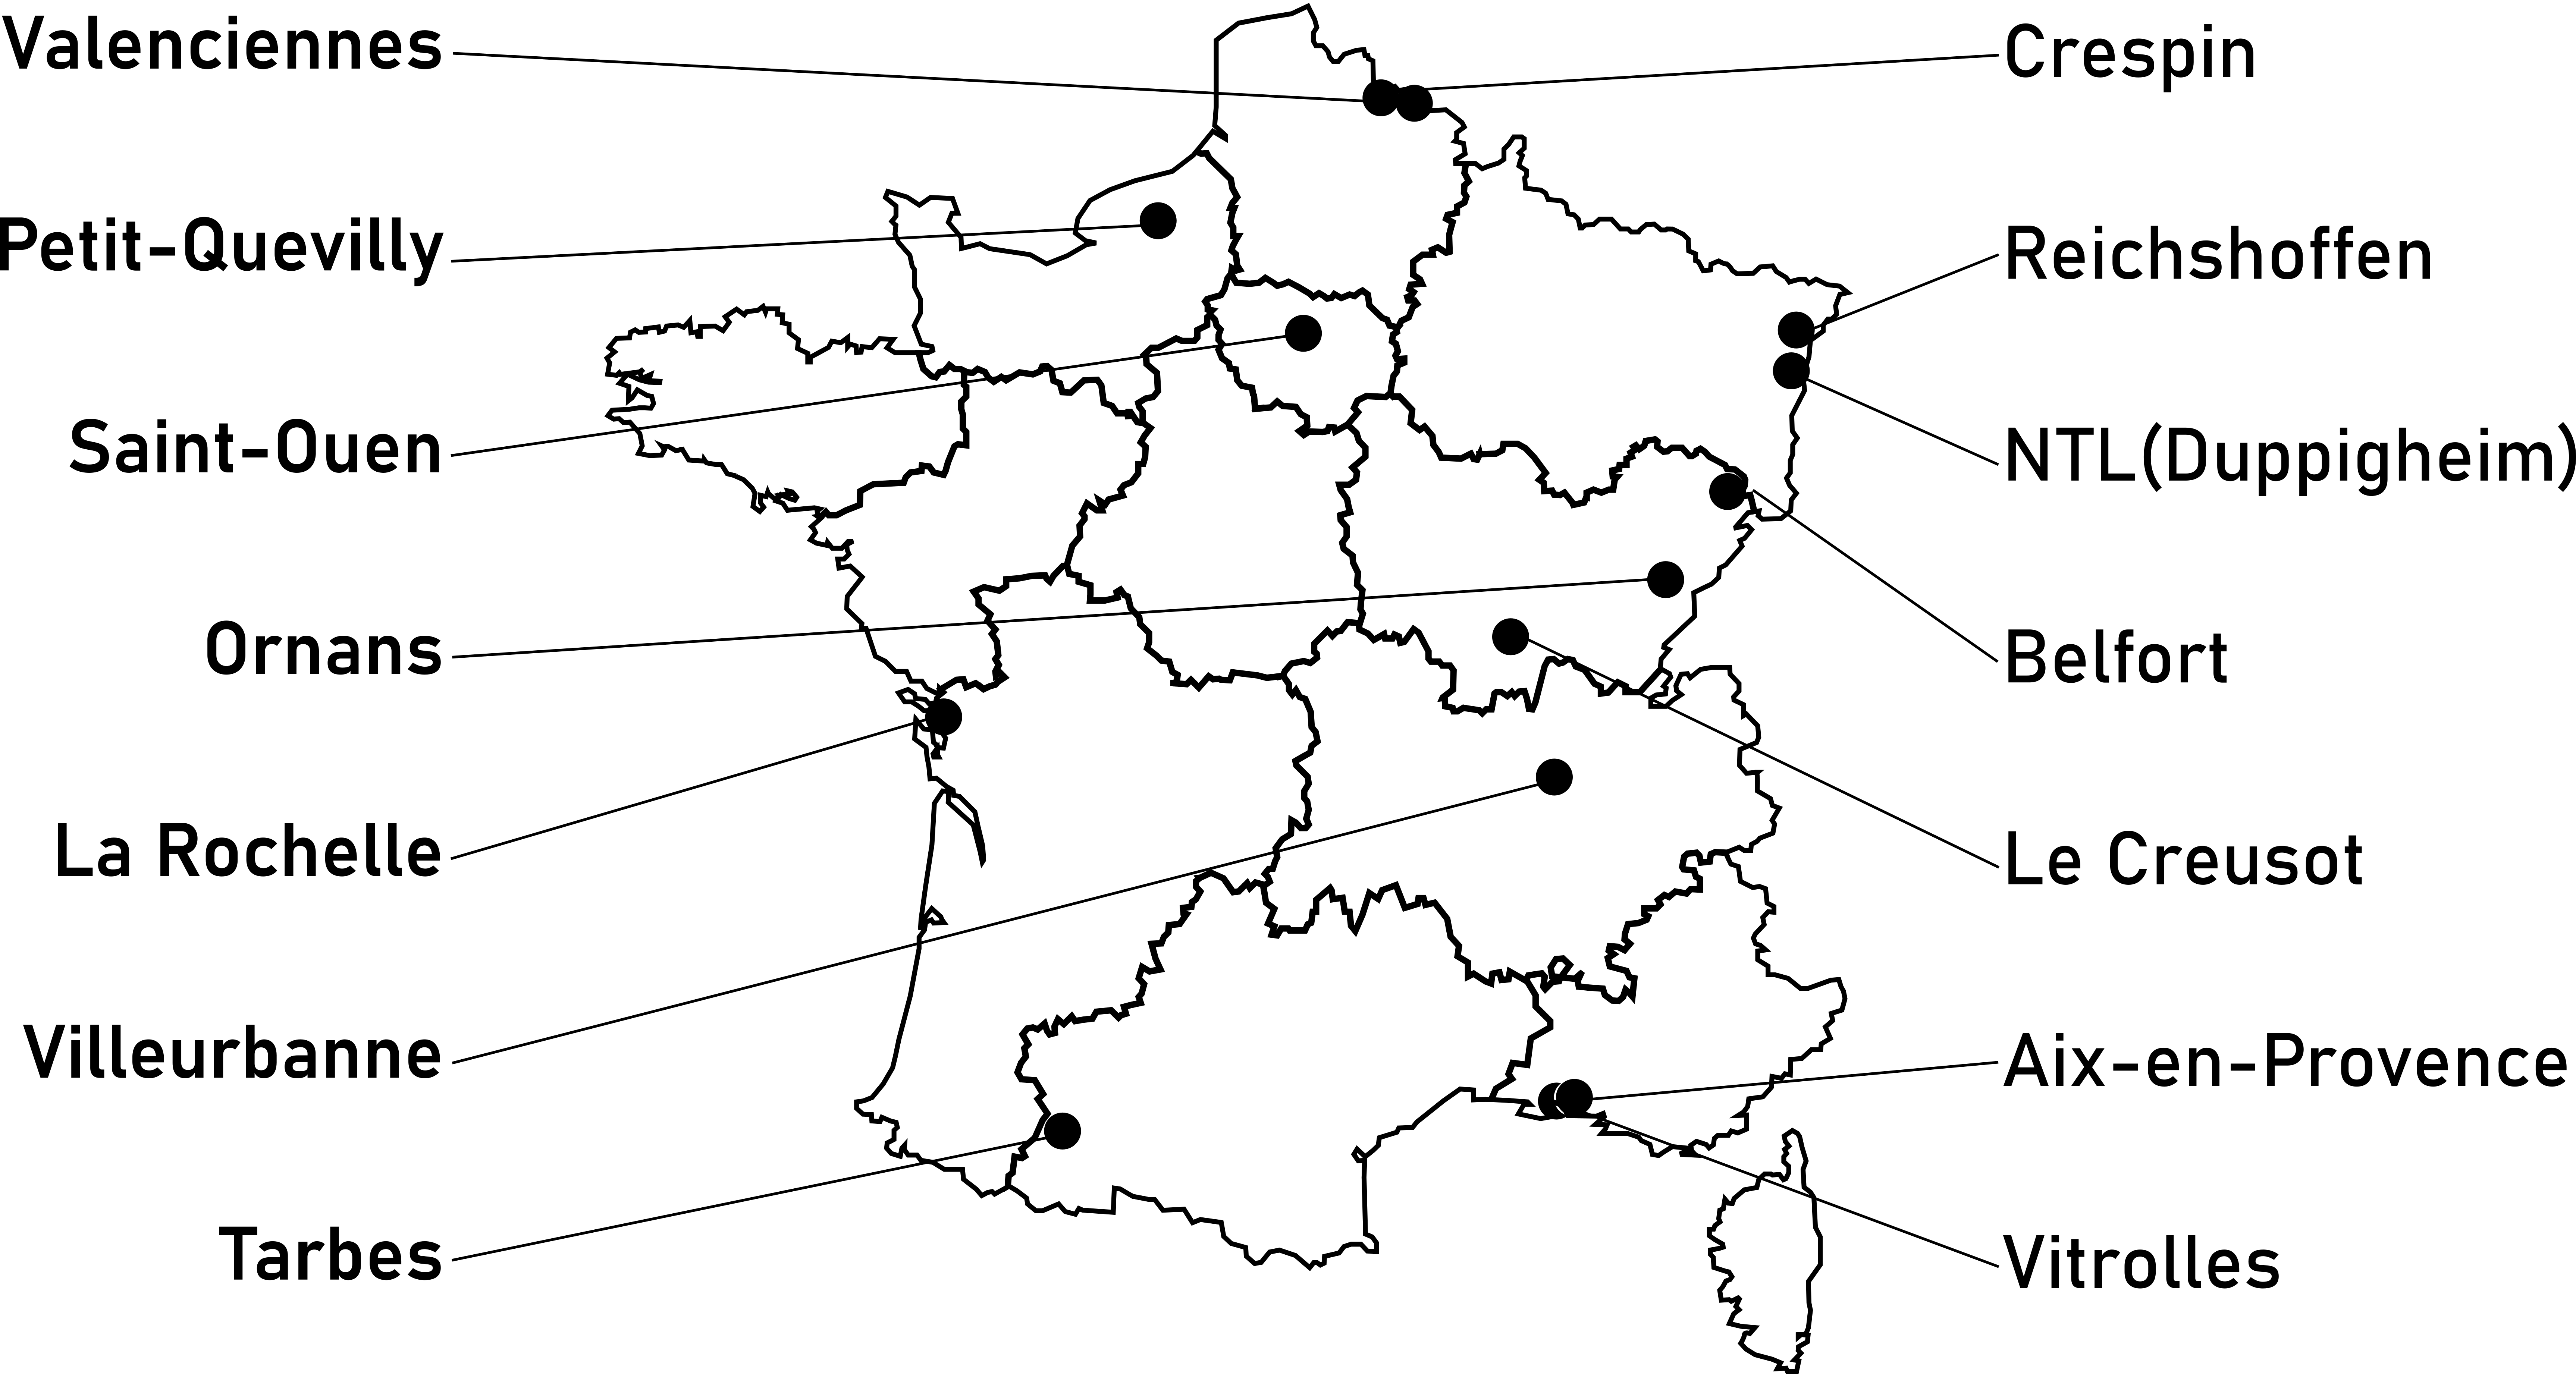
\includegraphics[width=0.9\linewidth]{carte_france} 
		\caption{Implantations françaises d' Alstom}
		\label{fig:carte}
	\end{wrapfigure}
	Alstom est une multinationale française spécialisée dans le secteur des transports, principalement ferroviaires.
	À l'origine Als-Thom, contraction d' "Alsace" et de "Thomson", devenue Alsthom, était le résultat de la fusion, réalisée en septembre 1928, d'une partie de la Société alsacienne de constructions mécaniques (SACM) basée à Mulhouse puis à Belfort, spécialiste de la construction de locomotives, et de la Compagnie française pour l'exploitation des procédés Thomson Houston (CFTH), société franco-américaine spécialiste des équipements de traction électrique ferroviaire et de la construction électromécanique.\\
	
	Elle devient Alsthom en 1932, puis Alsthom Atlantique en 1976, puis GEC-Alsthom en 1989 et Alstom depuis 1998. Avant 2016, le groupe Alstom comptait deux métiers, le transport et l'énergie, ce qui a changé lors du rachat de la branche Énergie par General Electric. Dorénavant Alstom concentre son activité dans le domaine des transports et en particulier le ferroviaire.\\
	
	Dernièrement, Alstom dispose de plus de 250 sites dans le monde dont 12 en France représentant 8500 collaborateurs. La majorité des implantations françaises présentent des activités de conception et de fabrication où chaque site évolue dans un domaine de compétence propre.  On peut notamment citer la succursale de Villeurbanne, spécialisée dans la conception et la fabrication des systèmes informatiques embarqués, ou bien celle de Ornans qui conçoit et fabrique des moteurs de traction ainsi que des alternateurs.\\
	
	En janvier 2021, Le groupe Alstom finalise le rachat de Bombardier Transport, la division ferroviaire de la multinationale canadienne Bombardier.\\
	
	A ce jour, le groupe est tourné vers l'éco-conception. Le train à hydrogène Coradia iLint et le bus Aptis sont présentés comme des alternatives sans émission de $CO_2$ aux trains à moteur thermique. L'automatisation du pilotage des trains est un autre enjeu important pour le groupe.\\
	
\pagebreak % PAGE BREAK !!! ------------------------------------------------- PAGE BREAK !!!
	
	\section{Site de Tarbes}
	C'est en 1932 que l'usine de la société des Constructions Électriques de France fusionne avec Alsthom.
	Entre 1921 et 1939, 596 locomotives dont 497 électriques furent construites dans l'établissement de Soues-Séméac.
	A la sortie de la seconde guerre mondiale où les activités ferroviaires furent arrêtées, le site voit diverses transformations et agrandissements qui seront poursuivis en 1957 avec une profonde réorganisation de la société.
	L'usine de Tarbes est divisée en groupes indépendants : département Traction chargé des moteurs et appareillages et le département diesel, fonderie et laboratoire.
	
	Jusque dans les années 1980, Alsthom arrête progressivement ses activités de fonderie, de fabrication de moteurs et de groupes électrogènes au profit du développement de l'électronique.
	On note un essor important dans les convertisseurs de puissance. Les anciens bâtiments sont convertis en salles blanches. Tarbes devient un site de référence dans la maîtrise des systèmes embarqués. En 1993, la direction de GEC Alsthom Transport décide de se réorganiser selon une logique de "produit".
	Tarbes se spécialise alors dans les projets de locomotives et les TGV. au cours des années 2010, les activités sont recentrées sur la Recherche et Développement.
	Le parc industriel est réaménagé pour accueillir les équipes R$\&$D (comptant ingénieurs et techniciens) qui représentent maintenant $80\% $ des effectifs.\\
	Aujourd'hui, le site de Tarbes développe plusieurs produits, dont notamment:
	\begin{itemize}
		\item chaîne de traction:
		Système qui convertit la puissance issue de la caténaire, ou d'une source embarquée, une batterie ou une pile à combustible, en puissance de traction et en puissances auxiliaires pour les équipements électriques ne contribuant pas directement à la mise en mouvement du train.
		\item modules de puissance:
		Sous ensemble des chaînes traction constituant un convertisseur de puissance. Ils comprennent les interrupteurs, leur circuit de commande et leur système de refroidissement. Les modules de puissance font l'objet de travaux de recherche et développement avec
		\begin{itemize}
			\item l'introduction des MOSFETs SiC (carbure de silicium), permettant une fréquence de commutation plus élevée et d'économiser de l'énergie.
			\item la numérisation des cartes de commande, permettant de d'augmenter la fiabilité des convertisseurs et le diagnostic des modules de puissance.
			\item le développement du refroidissement par boucle à pompage capillaire (CPL), permettant de réduire le niveau de bruit, les coûts de maintenance et la consommation d'énergie.
		\end{itemize}
		\item appareillages :
		Il s'agit de disjoncteurs ultrarapides, des contacteurs et des sectionneurs utilisés pour la protection, l'isolation et la reconfiguration des circuits de puissance des chaînes de traction ou des installations au sol.\\
		Le site de Tarbes conçoit et fabrique une large gamme de produits dont le courant nominal s'étend de 250A à 8kA et de 750V à 3kV en continu et jusqu'à 25kV en alternatif.\\
	\end{itemize}
	

	\chapter{Contexte et objectifs du stage}

	
	\section{Contexte}
\subsection{Evolution de la technologie des tractions ferroviaires}
	Historiquement, les caténaires délivraient principalement du courant continu et les trains utilisaient un moteur de type série-continu. C’était le moteur à courant continu le plus apte à la traction ferroviaire du fait de son fort couple au démarrage (2200 kW). Avec une très faible résistance électrique ($\leq 1\Omega$), ces moteurs causent une montée brutale du courant au démarrage et à l'arrêt. Il était alors nécessaire d'incorporer des résistances dans le circuit de traction pour dissiper de cette énergie électrique en effet Joule. La température de ces résistances de démarrage étant à l'image du courant, Alstom a cherché à changer sa façon de gérer l'énergie.\\
	
	C'est au cours des années 1970 qu'on équipe les tractions de hacheurs de courant à thyristor ce qui permet de remplacer les rhéostats de démarrage, il s'agit un avantage capital, mais la commande de ces convertisseurs est encore analogique. Il faut attendre 1989 pour voir l'arrivée des commandes numériques et des systèmes informatiques embarqués. Le moteur série-continu disparait au profit des machines synchrones pilotées par des onduleurs fonctionnant eux aussi avec des thyristors.\\
	
	La locomotive DB36000 (1996)s utilisa pour la première fois un moteur asynchrone. Sa puissance est de 1200kW pour une masse de 1350kg. Sous caténaire monophasée, l'énergie est fournie à un convertisseur 4 quadrants, le Pont Mixte à Commutation Forcée (PMCF) qui utilise des modules IGBT.\\
	
	Depuis, les chaînes de tractions sont structurées avec un PMCF et un onduleur pour chaque secondaire du transformateur principal. La figure \ref{schema:traction} montre le schéma de principe d'une chaîne de traction. Cette structure est générique et adaptée en fonction du besoin.\\

		\begin{figure}[h]	
		\begin{center}			
		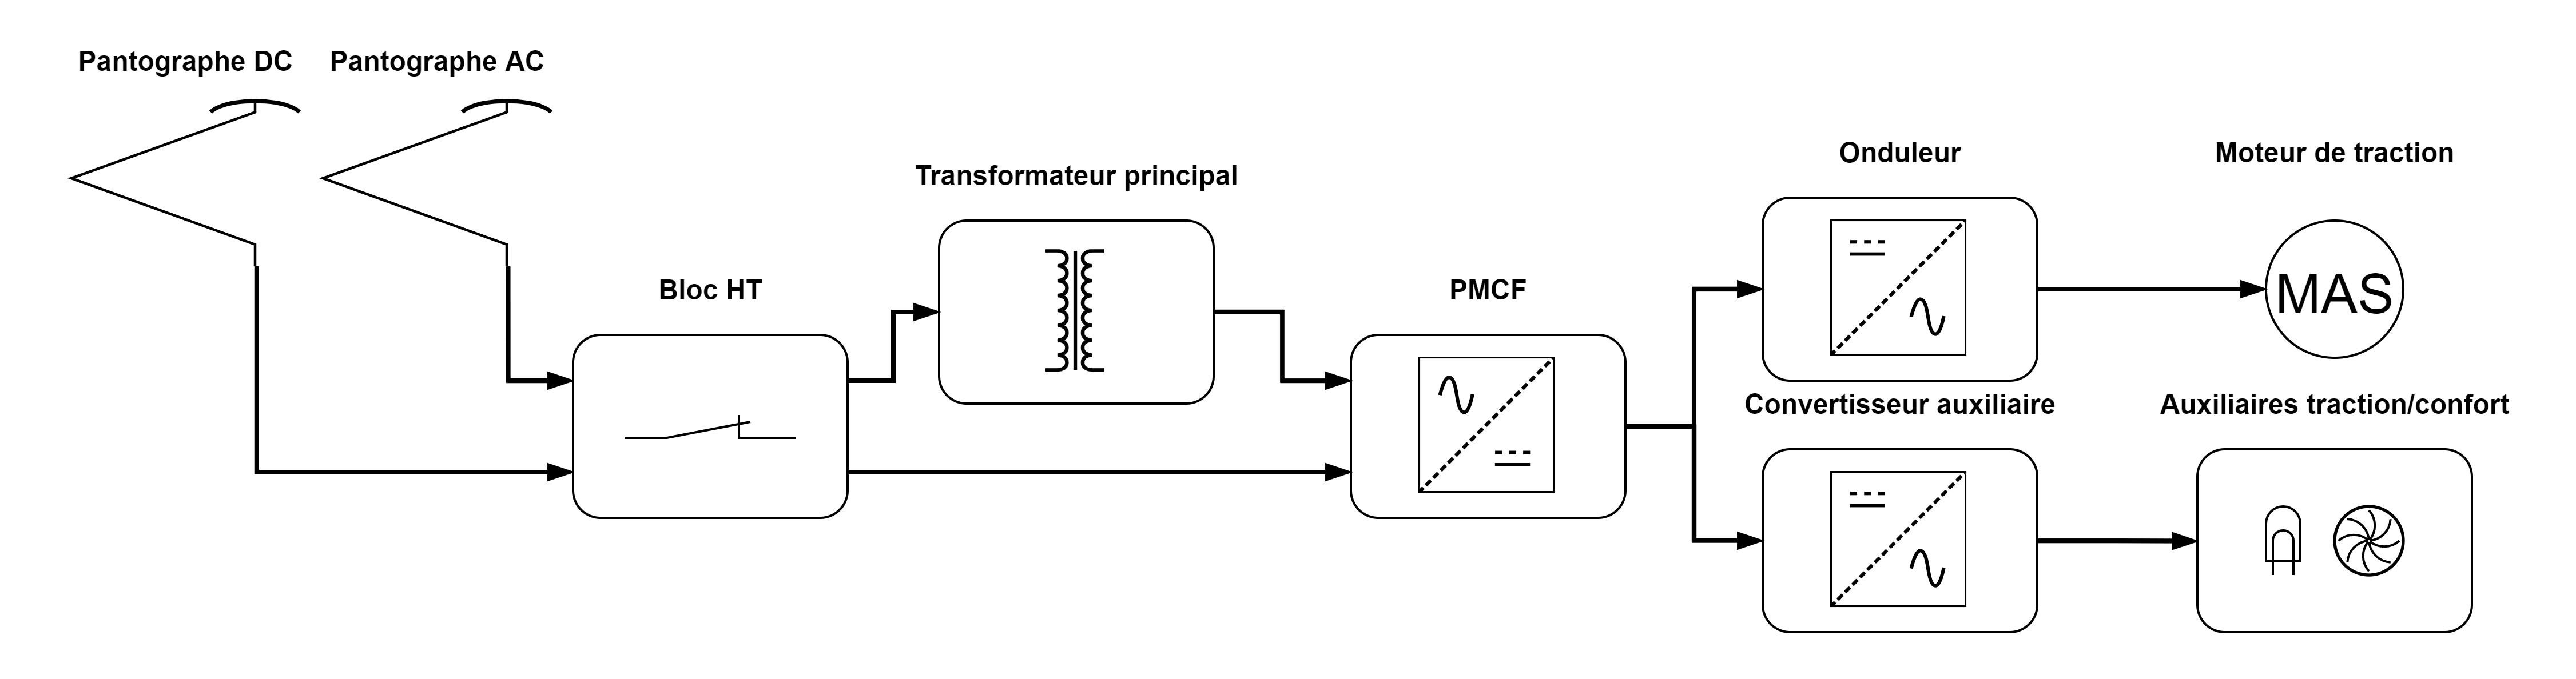
\includegraphics[width=0.8\textwidth]{chaine_traction}
		\caption{principe d'une chaîne de traction ferroviaire}
		\label{schema:traction}				
		\end{center}
		légende de la figure \ref{schema:traction}:
		\begin{itemize}
	\item Le bloc Haute Tension fait la séparation
	\item Le transformateur principal (TFP) abaisse le niveau de tension
	\item Le PMCF redresse la tension alternative ou hache la tension continue. Il permet aussi le freinage par récupération.
	\item L'onduleur de traction fournit un courant au moteur en fonction de la consigne de vitesse.
	\item L'onduleur auxiliaire alimente les fonctions ne contribuant pas directement de la mise en mouvement du train. On distingue les auxiliaires de traction ayant un rôle dans la chaîne de traction (ventilations, charge de batteries, ...) des auxiliaires de confort remplissant d'autres rôles dans le train (éclairage, climatisation, ...).
\end{itemize}
		\end{figure}



\subsection{Calculateur TCUs}	
	Le pilotage et la surveillance des PMCFs, onduleurs, hacheurs et capteurs sont assurés par le TCU (Traction Control Unit). Ce calculateur est générique et son programme doit être adapté à chaque projet. La conception et la programmation de ce logiciel est la mission principale du service Contrôle-Commande.\\
	Afin de certifier le logiciel pour qu'il soit utilisé dans un train, il est nécessaire de le tester. A l'origine, les tests sont effectués sur des bancs de test reproduisant la chaîne de traction à échelle réelle. Néanmoins, cette méthode à pour inconvénient d'être très couteuse en temps et en matériel.
\subsection{Simulation HIL}	
	La simulation Hardware-In-the-Loop (HIL) est une technique remédiant aux limitations du banc de test. Le but est de vérifier et certifier la fonctionnalité, la performance, la qualité et la sécurité d'un calculateur. Pour ce faire, le comportement dynamique du système réel est converti en un modèle logiciel qui est exécuté sur un simulateur en temps réel (cf. figure \ref{schema:hil}).
	L'équipement est connecté aux entrées/sorties du simulateur qui émule le fonctionnement des actionneurs et capteurs réels. 
	%En recréant le monde réel, l'équipement croit être connecté au système physique.
	 Une grande flexibilité dans le test des équipements de traction sous n'importe quelle condition de fonctionnement est alors possible.

	\begin{wrapfigure}{l}{0.5\textwidth}
		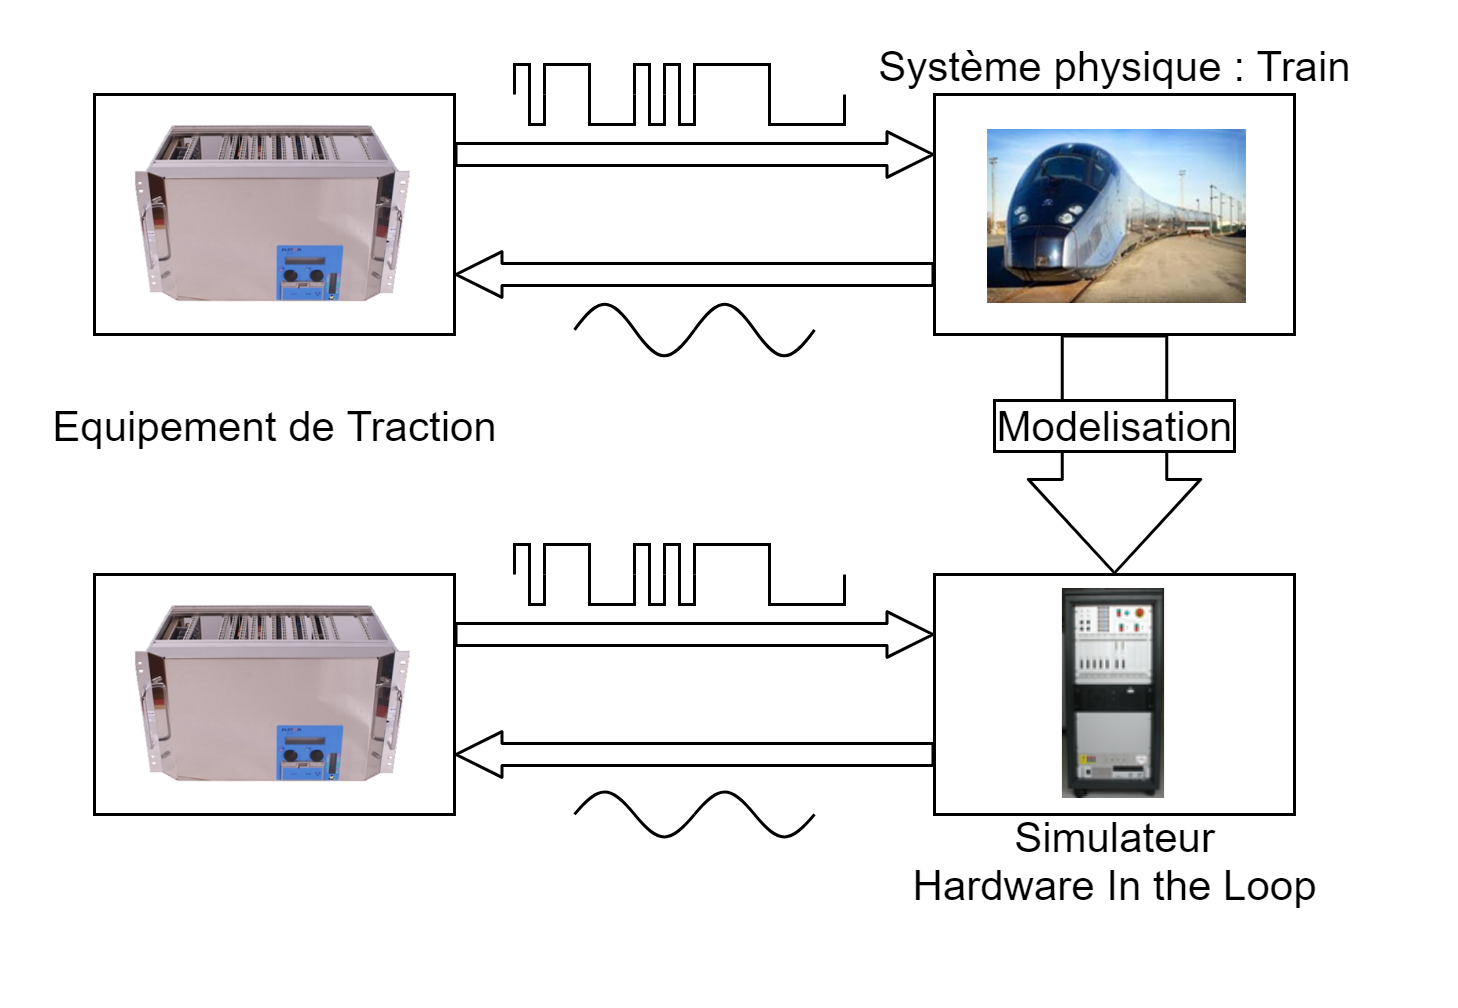
\includegraphics[width=0.5\textwidth]{schema_hil}
		\caption{fonctionnement d'un simulateur HIL}
		\label{schema:hil}
	\end{wrapfigure}
	
	On peut réaliser deux types de simulations selon le matériel à simuler (cf. figure \ref{schema:sitra}).\\ 
	Les appareils basse tension et les auxiliaires de traction utilisent la simulation \textbf{lente}. Les modèles sont programmés au travers du logiciel ControlBuild en langage Grafcet (SFC), en langage à contact (LD) ou en langage textuel de haut niveau (ST). Ce type de simulation est exécutée périodiquement toutes les 50ms lui permettant d'être réalisée sur simulateur ou entièrement sur PC (dans ControlBuild).\\ 
	La simulation \textbf{rapide} est utilisée pour les éléments d'électronique de puissance ainsi que pour le modèle cinématique du train (vitesses, efforts) et le contrôle du freinage. Les dynamiques très rapides de ces systèmes ne permettent pas de simuler sur pc.
	\begin{figure}[h]			
		\centering
		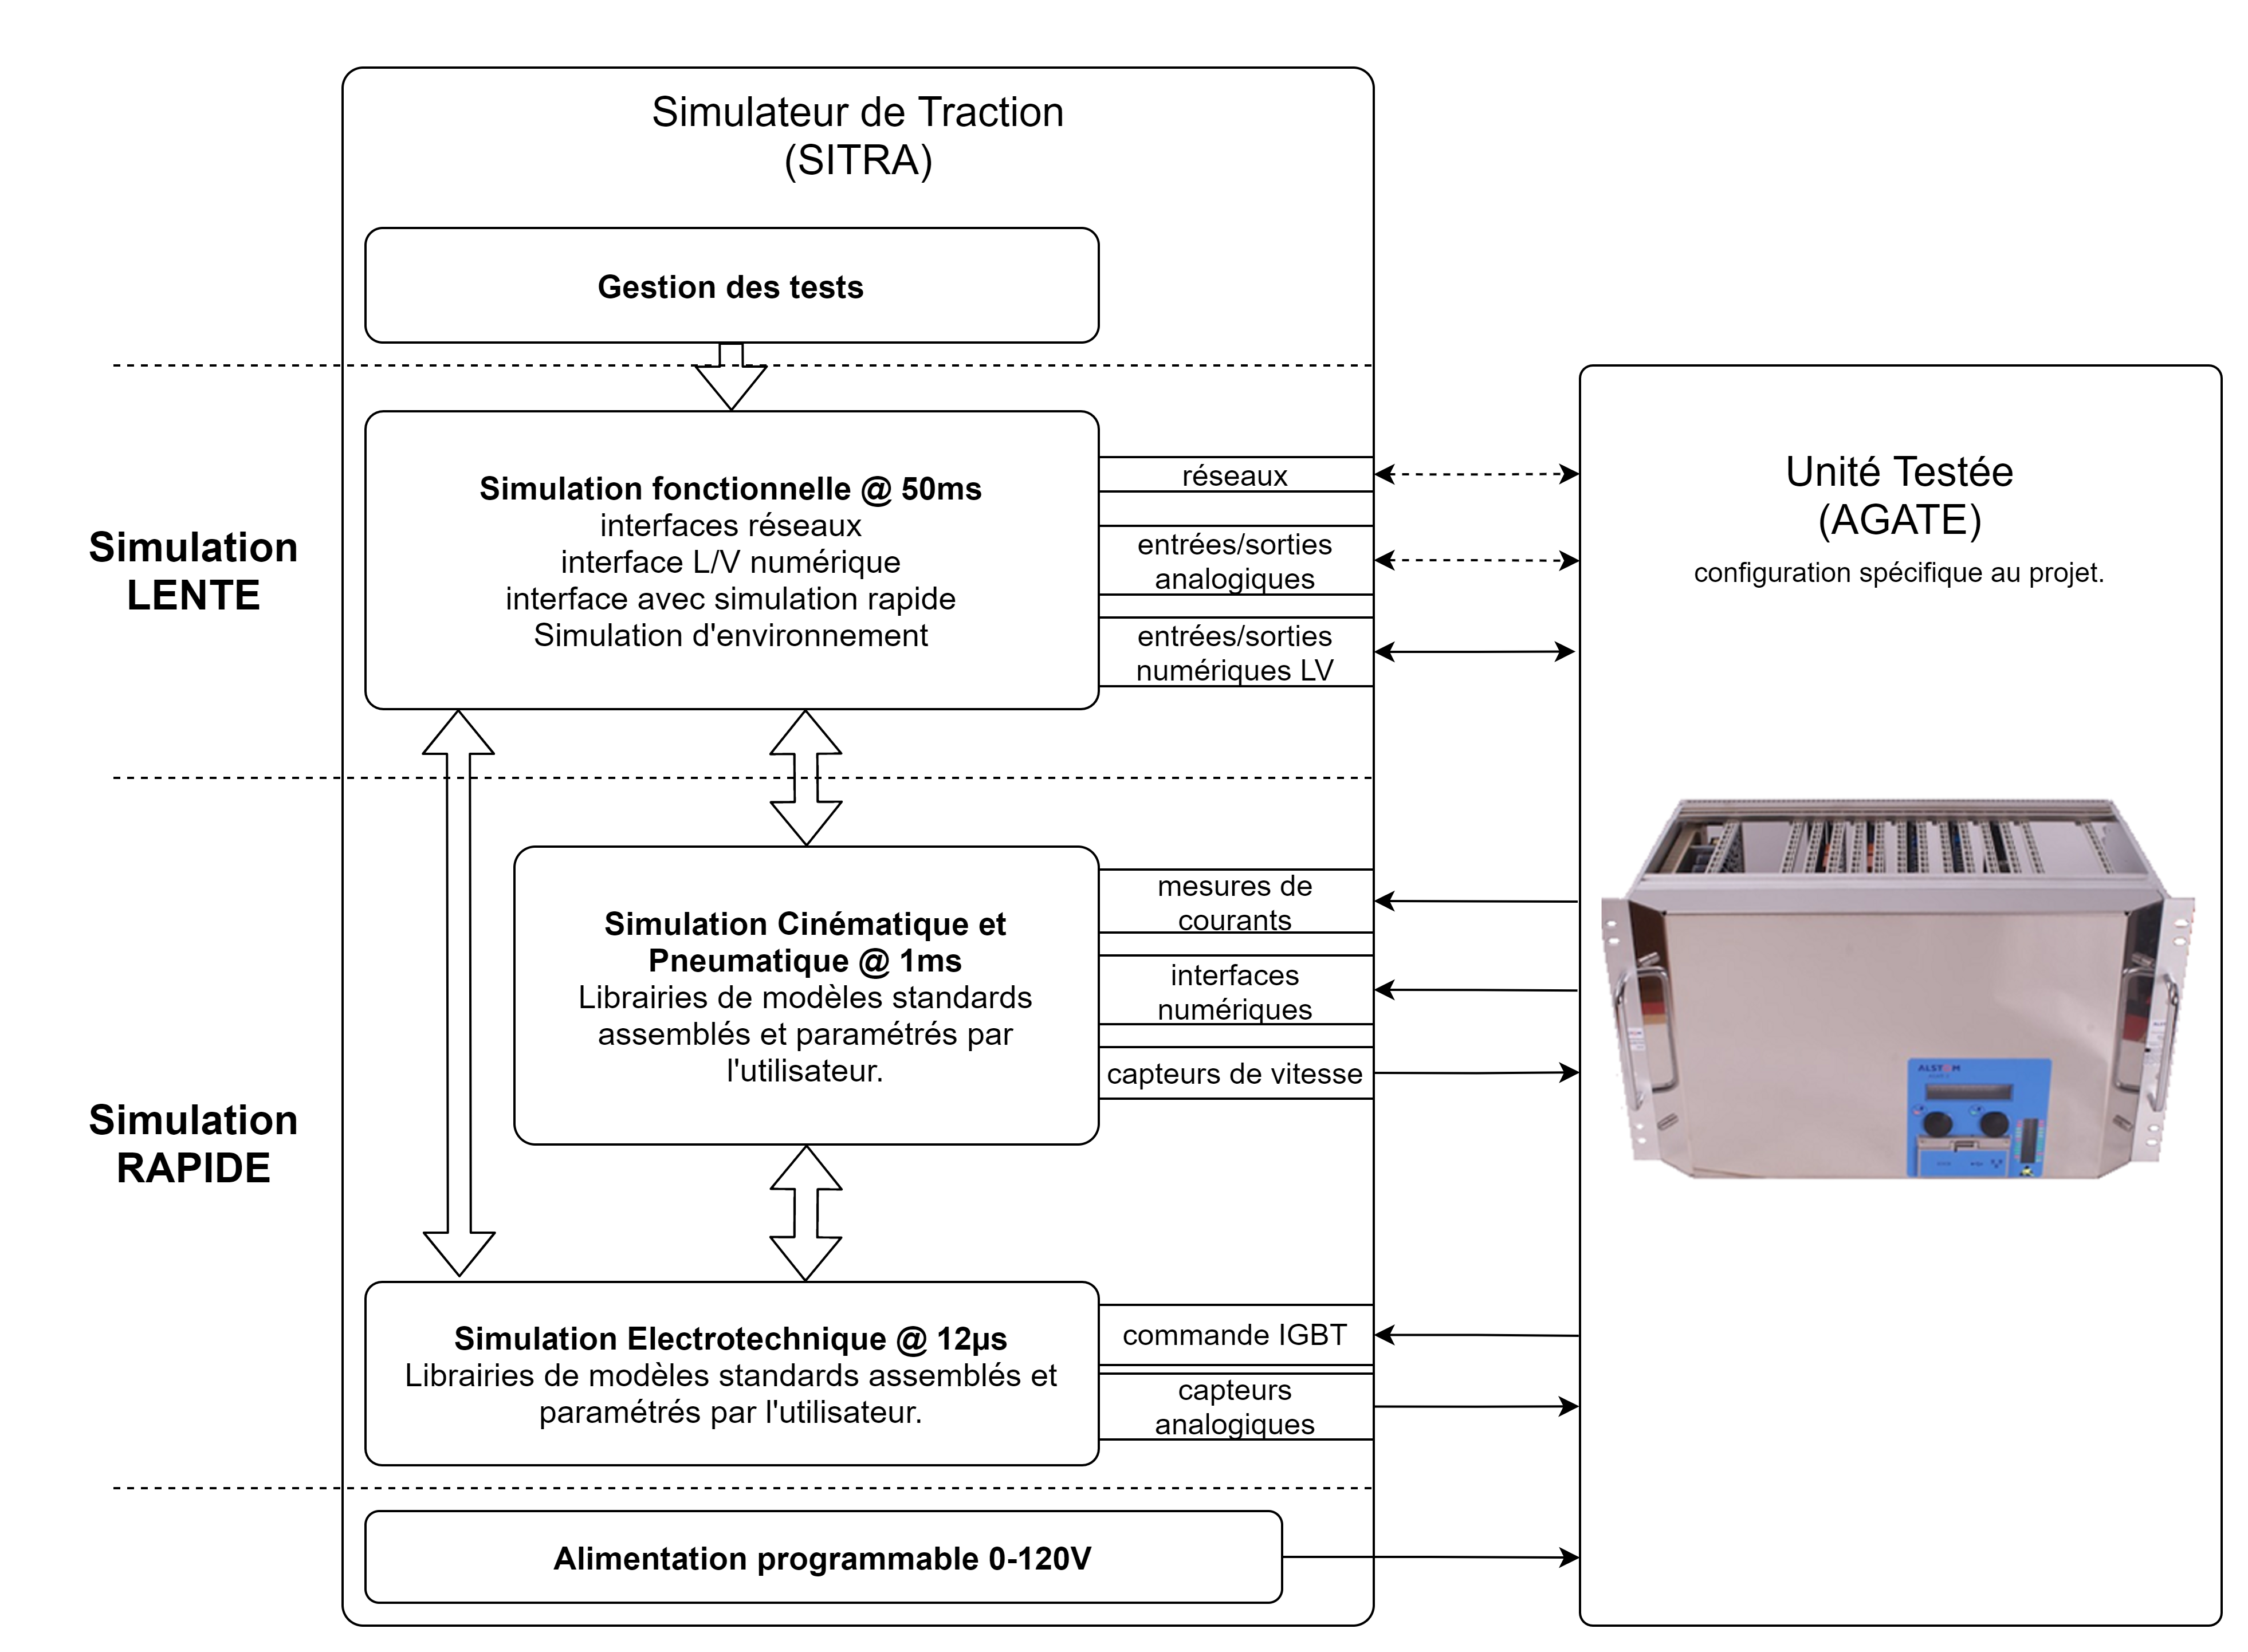
\includegraphics[width=0.80\textwidth]{schema_sitra}
		\caption{architecture du simulateur de traction}
		\label{schema:sitra}
	\end{figure}
	Le but de ce stage est de développer des applications (composants) ControlBuild modélisant le comportement thermique d'un rhéostat de freinage ainsi que d'un transformateur de puissance en utilisant l'analogie entre circuit électrique et circuit thermique. On se place donc dans le contexte d'une simulation lente.\\
	
\pagebreak % PAGE BREAK !!! ------------------------------------------------- PAGE BREAK !!!

	\section{Sujet principal: Modèle thermique du Rhéostat de Freinage}
	Le freinage rhéostatique est une technique visant à dissiper l'énergie cinétique du moteur de traction en effet Joule. Elle est utilisée lorsque le freinage à récupération, une autre méthode permettant de renvoyer l'énergie sur le réseau, n'est pas utilisable. La puissance dissipée dans le rhéostat est à l'image de l'effort de freinage. Cette méthode a l'avantage d'être autonome donc de pouvoir fonctionner à disjoncteur ouvert et par conséquent, il ne renvoie pas d'harmoniques sur le réseau.\\
	\begin{figure}[h]			
		\centering
		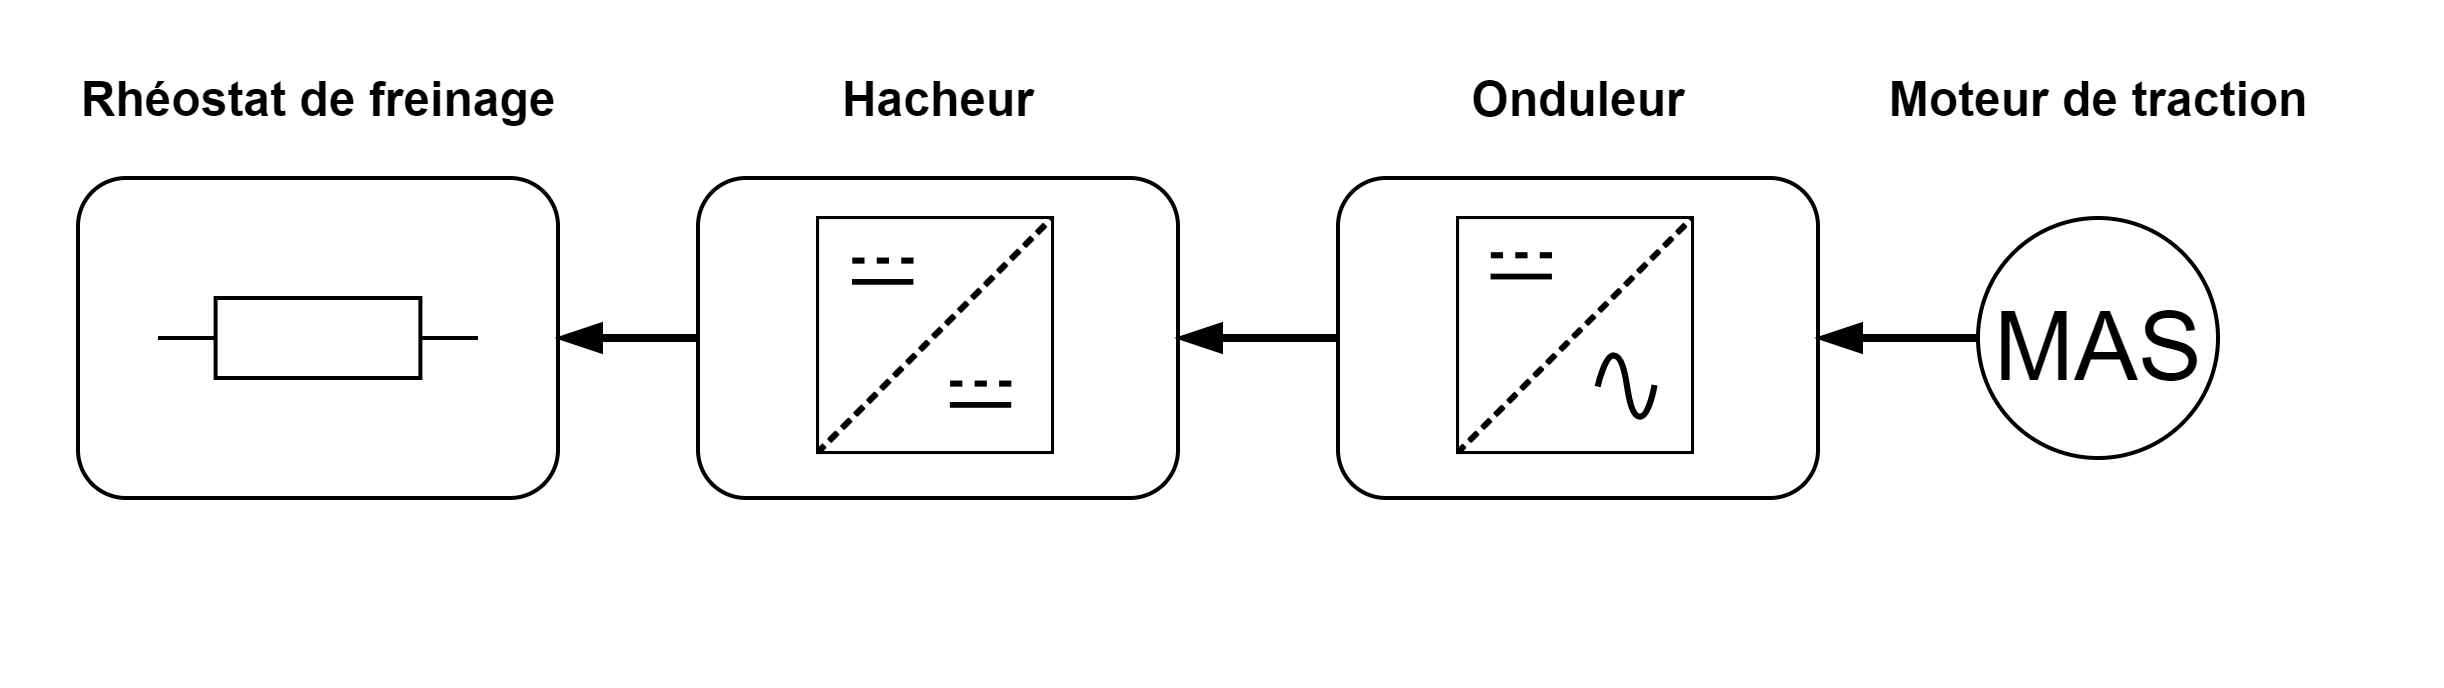
\includegraphics[width=0.60\textwidth]{rheostat_freinage}
		\caption{principe du freinage rhéostatique}
		\label{schema:rheo}
	\end{figure}
	Jusqu'à présent, un modèle thermique du hacheur ainsi que du rhéostat de freinage sans variation dynamique de la résistance sont utilisés. En effet, la valeur du rhéostat en Ohm augmente avec la température. Or, un tel changement entraîne une modification de l'effort de freinage.\\
	Pour évaluer l'effet de ces changements, l'équipe contrôle-commande doit manuellement ajuster la résistance du rhéostat en paramètre d'entrée du modèle. Afin de faciliter la simulation du rhéostat freinage et d'obtenir une image plus représentative de l'échauffement, on souhaite réaliser un nouveau modèle calculant la résistance corrigée du rhéostat ainsi que sa température en fonction du courant qui le traverse.

\pagebreak % PAGE BREAK !!! ------------------------------------------------- PAGE BREAK !!!

	\section{Sujet secondaire: Modèle thermique du Transformateur principal}
	Le transformateur principal a pour rôle de convertir la tension alternative provenant de la caténaire (25kV) en une tension de plus faible niveau (1 kV par secondaire, 4 secondaires) avant qu'elle soit redressée et utilisée dans la chaîne de traction.
	Le transformateur principal voit donc beaucoup de puissance passer et génère des pertes qu'il est nécessaire d'évacuer.
	Dans notre application, le transformateur est contenu dans un circuit d'huile forcé par une pompe.
	L'huile est ensuite refroidie par un échangeur thermique à ailettes. L'échangeur est lui-même refroidi par une ventilation.\\
	Comme dans le sujet précédent, il est nécessaire d'observer la température des éléments actifs (dissipant de la puissance) et de l'huile dans le circuit de façon à ne pas endommager le transformateur (i.e. dégradation des isolants en cas de surchauffe). Le second objectif du stage est donc de réaliser un modèle thermique du transformateur principal.\\
	
	
	\section{Spécification de la solution}
	
	Les modèles sont réalisés en utilisant l'analogie entre thermique et électricité. On considère uniquement la conduction et la convention forcée pour modes de transferts thermiques. Cette hypothèse permet de limiter la modélisation à l'application des lois de Fourier et de Newton.\\
	
	On cherche à obtenir une valeur température résumant le comportement de chacun des systèmes. Le but étant de faire de la supervision, il n'est pas utile d'utiliser une méthode de simulation détaillée comme c'est le cas avec l'analyse par éléments finis.\\
	
	Les modèles thermiques sont programmés en \textbf{Structured Text} sous la plateforme \textbf{ControlBuild} et doivent s'intégrer dans les projets de simulation existants.\\
	
	Voici la liste des exigences à laquelle doivent répondre les programme :
	
	\begin{itemize}
		\item compatibilité avec le reste de la simulation.
		\item respect des règles de codages.
		\item programme prévu pour un fonctionnement continu en temps réel.
		\item prise en compte des différents états du système (vitesse de ventilation).
		\item intégration de plusieurs modes de forçage pour effectuer des tests sur le modèle
	\end{itemize}
	
	Avec la description de la spécification, on peut maintenant passer à la réalisation du sujet principal.
	\chapter{Étude des problèmes, solutions, mise en œuvre des résultats (10 pages)}
	
	
	\section{Introduction aux transferts de chaleur}
	Un transfert de chaleur est le transport d'énergie thermique d'une région vers une autre. Pour qu'un transfert se produise, il faut observer une différence de température entre ces régions. La chaleur circule toujours de la région chaude vers la région froide. Un transfert de chaleur peut se produire sous trois modes distincts : conduction, convection et radiation.\\
	La conduction est le transfert d'énergie thermique entre des solides ou fluides à l'arrêt. La convection est le mode par lequel l'énergie thermique est transférée depuis ou vers un fluide en contact avec une surface solide. La radiation est le mode par lequel l'énergie est transférée sous forme d'ondes électromagnétiques. Le modèle de rhéostat n'utilisera que la conduction thermique tandis que le modèle de transformateur considèrera la conduction ainsi que la convection.\\
	La conduction thermique est décrite par la loi de Fourier. Elle dit que dans un milieu homogène le flux de chaleur local est proportionnel à la différence de température. En régime établi, le flux thermique au travers d'une surface S vaut :
	\begin{equation}
		\phi = \frac{\lambda S}{e} \times (T_{froid} - T_{chaud} ) 
	\end{equation}
	
	Avec $ \phi $ le flux thermique en $ W $, $ \lambda $ la conductivité du milieu en $ W m^{-1} K^{-1} $ et $ e $ l'épaisseur du milieu en m.\\
	
	La loi des nœuds et la loi des mailles sont applicables pour l'analyse des circuits linéaires et non-linéaires. Le flux de chaleur étant analogue au courant électrique et la température étant analogue à la tension, on peut appliquer ces lois aux circuits thermiques.\\
	
	La convection thermique est le terme utilisé pour décrire le transfert entre une surface et un fluide en
	mouvement. Le taux de transfert thermique par convection est fonction de la géométrie de la surface et de sa 
	température, mais dépend aussi des propriétés physiques du fluide. Dans le cas d'un flux externe forcé, comme pour l'huile du circuit de refroidissement dans le transformateur,  la loi de Newton nous dit que le taux de transfert est proportionnel à la différence entre la température de la surface. Son expression est très semblable à la loi de Fourier:
	
	\begin{equation}
		\phi = h_c S \times (T_{froid} - T_{chaud}) 
	\end{equation}
	
	Avec $ \phi_s $ le flux de chaleur convectif en $ W $, $h_c$ le coefficient de transfert thermique en $ W 			m^{-2} K^{-1} $ \\
	
	Les deux équations présentées sont analogues à la loi d'Ohm. On peut faire le lien entre les grandeurs:
	\begin{center}
		\begin{tabular}{|l||l|}
			\hline
			Thermique                 & Electricité                \\
			\hline
			température (K)          & tension (V)                 \\
			\hline
			flux thermique (W)        & courant (A)                 \\
			\hline
			conductivité ($WK^{-1}$) & conductance ($\Omega^{-1}$) \\
			coefficient de convection &                             \\
			\hline
		\end{tabular}
	\end{center}
	
	\section{Modèle du rhéostat de freinage}
	
	\subsection{Début du projet, revue des données techniques}
	Dans ma démarche, j'ai en premier lieu trouvé pertinent de consulter la documentation fournie par le constructeur. Le but est de trouver des informations qui peuvent guider la conception du modèle. On trouve notamment une valeur de résistance électrique donnée pour une température de 20°C de 1.31$\Omega$. On se rend aussi compte que cette valeur est affectée par la température, le coefficient de température du rhéostat vaut $5.5\times10^{-4}$.\\
	
	La fiche technique renseigne aussi plusieurs valeurs de résistances thermiques ($R_{th}$),ainsi qu'une valeur de capacité thermique ($C_{th}$) dérivée de la chaleur spécifique en fonction de la vitesse de ventilation: 
	
	\begin{center}
		\begin{tabular}{|c|c|c|}
			\hline
			vitesse de ventilation & Résistance Thermique (°C/kW) & Capacité Thermique (J/°C) \\
			\hline
			sans ventilation       & 20.76                        & 36 370                    \\
			\hline
			petite vitesse         & 1.403                        & 36 370                    \\
			\hline
			grande vitesse         & 0.797                        & 36 370                    \\
			\hline
		\end{tabular}
	\end{center}
	
	La baisse de température due a la ventilation est modélisée par une réduction de Rth. La capacité thermique n'est pas modifiée par la ventilation.\\ %car elle dépend principalement de la masse du système.
	Le document dispose aussi d'une section de simulation thermique. On y trouve plusieurs réponses indicielles pour les différentes vitesses de ventilations.

	\subsection{Modèle sous forme de filtre RC}
	Selon les données collectées, on se rend compte que le circuit thermique peut être vu comme un filtre passe bas RC. La tension à l'entrée de ce filtre qu'on appelle \textbf{$T_{cible}$} est trouvée en appliquant la loi de Fourier:
	\begin{equation}
	T_{cible} = I_{RH} * R_{RH} * R_{Th} + T_{amb}
	\end{equation}
	avec $I_{RH}$ le courant traversant le rhéostat, $R_{RH}$ la résistance électrique du rhéostat, $R{Th}$ la résistance thermique du rhéostat et $T_{amb}$ la température ambiante.\\
	
	La loi de conduction thermique étant analogue à la loi d'Ohm, on peut représenter le circuit thermique équivalent du système:
	\begin{figure}[h]				
		\centering
		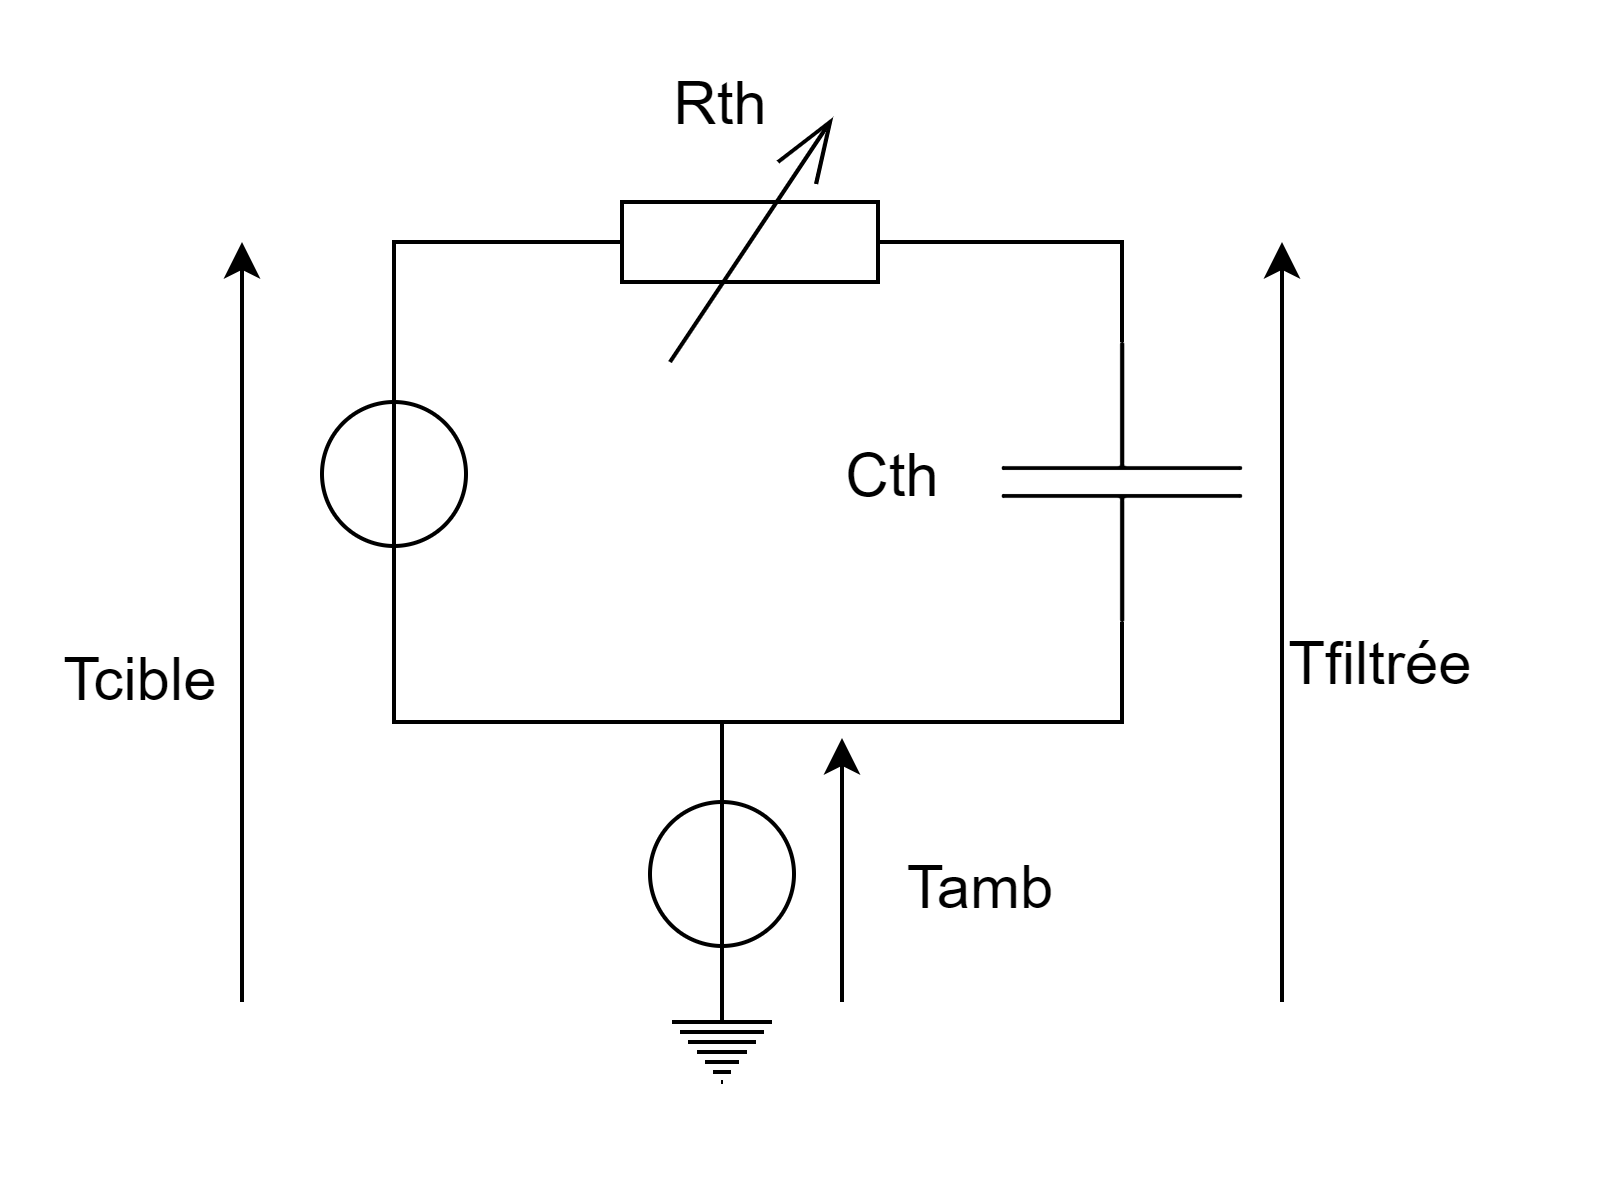
\includegraphics[width=0.4\textwidth]{schema_rcth}
		\caption{filtre analogique thermique du premier ordre}
		\label{schema:rcth}			
	\end{figure}
	
	En regardant ce circuit, on peut imaginer que la base de temps du filtre va changer en fonction de $R_{th}$ et donc en fonction de la vitesse de ventilation.\\
	
	Dans le contexte d'un programme exécuté en continu, on utilisera un filtre à réponse impulsionnelle infinie (RII) plutôt que la fonction de transfert du filtre. Un filtre RII est récursif et utilise la valeur de sortie précédente pour effectuer le calcul suivant, son expression est:
	$$ y(n) = b_0 \times x(n) + a_1 \times  y(n-1) $$ 
	Avec  $ a_1 = \frac{\tau}{\tau + Te} $ et $ b_0 = \frac{Te}{\tau + Te} $
	
	\pagebreak % PAGE BREAK !!! ------------------------------------------------- PAGE BREAK !!!
	
	\subsection{Correction de la résistance électrique}
	
	\begin{wrapfigure}{r}{0.4\textwidth}
		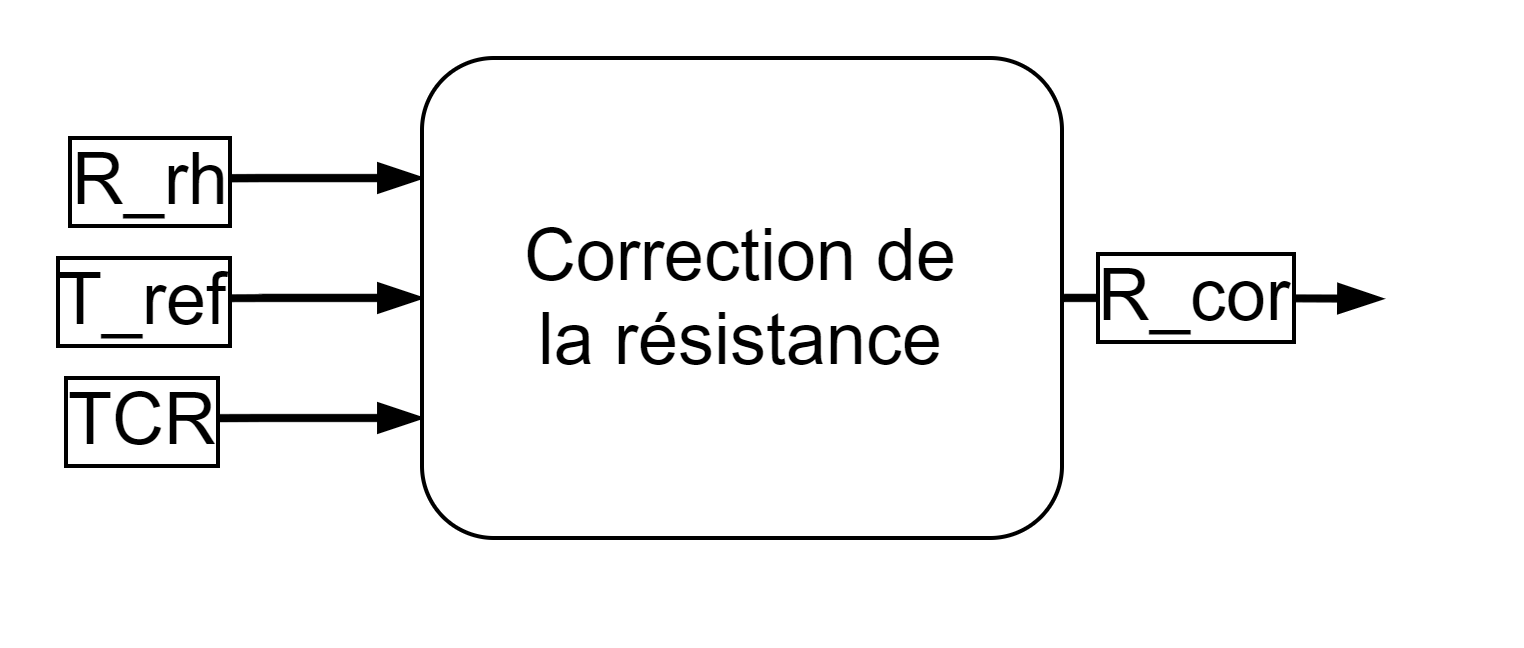
\includegraphics[width=0.4\textwidth]{R_cor}
		\caption{correction de la valeur de résistance}
		\label{schema:r_cor}
	\end{wrapfigure}
	On a vu dans la présentation du sujet que la résistance électrique du rhéostat dépend de la température. La valeur corrigée de cette résistance est donnée par : $ R_{cor} = R_{RH} \times TCR \times T_{filtree} + R_{RH}  $ avec TCR le coefficient de température de la résistance (Temperature Coefficient of Resistance), $T_{filtree}$ la température en sortie du filtre.\\
	
	On récrit cette expression pour obtenir une fonction de la forme $y = ax + b$ où $b = \frac{R_{RH}}{TCR \times T_{ref} + 1} $ et $a = TCR $ \\
	
	Cette écriture a l'avantage d'être plus pratique dans l'optique de programmer cette fonction puisqu'elle comprend la température de référence $T_{ref}$ à laquelle la résistance $R_{RH}$ est mesurée (cf. figure \ref{schema:r_cor}).
	
	
	
			
	
	\subsection{Réalisation d'un modèle sous OpenModelica}
	\begin{wrapfigure}{r}{0.3\textwidth}
		
\includegraphics[width=0.9\linewidth]{logo_openmodelica} 
		\caption{openModelica}
		\label{fig:logo_om}
	\end{wrapfigure}
	Avant de réaliser le code sous ControlBuild, je souhaite créer un premier modèle dans un logiciel de simulation multiphysique avec une interface graphique permettant la saisie de diagrammes en blocs.\\
	La motivation derrière ce besoin est que ControlBuild ne permet que de visualiser les valeurs instantanées des variables, alors qu'il est préférable d'afficher un graphe fonction du temps, permettant de connaître la tendance globale d'un système lent comme c'est le cas en thermique.\\
	
	La recherche d'un tel logiciel a finalement abouti sur \textbf{OpenModelica}. Il s'agit d'un programme de simulation OpenSource basé sur Modelica, un langage de modélisation orienté objet créé en 2000.\\
	
	OpenModelica rend très facile la création de nouveaux blocs à partir de blocs primitifs, ce qui a comme bénéfice de rendre un diagramme plus lisible.\\
	
	Dans un premier temps, je crée un bloc "TEMP RH" qui calcule une loi de Fourier pour donner une Température Cible qui passe par le filtre numérique dont je calcule les coefficients.\\
		
	
	\begin{figure}[h]
		
		\begin{subfigure}{0.5\textwidth}
			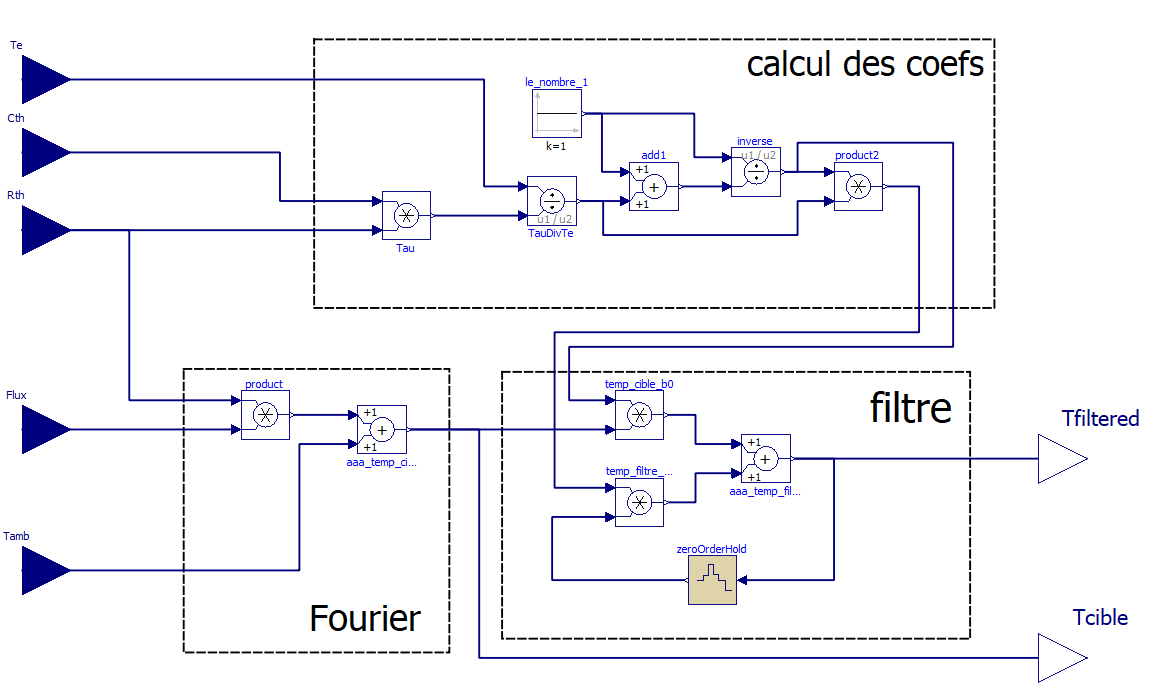
\includegraphics[width=0.9\linewidth]{rh_fourier} 
			\caption{Vue du contenu du bloc}
			\label{fig:subim1}
		\end{subfigure}
		\begin{subfigure}{0.5\textwidth}
			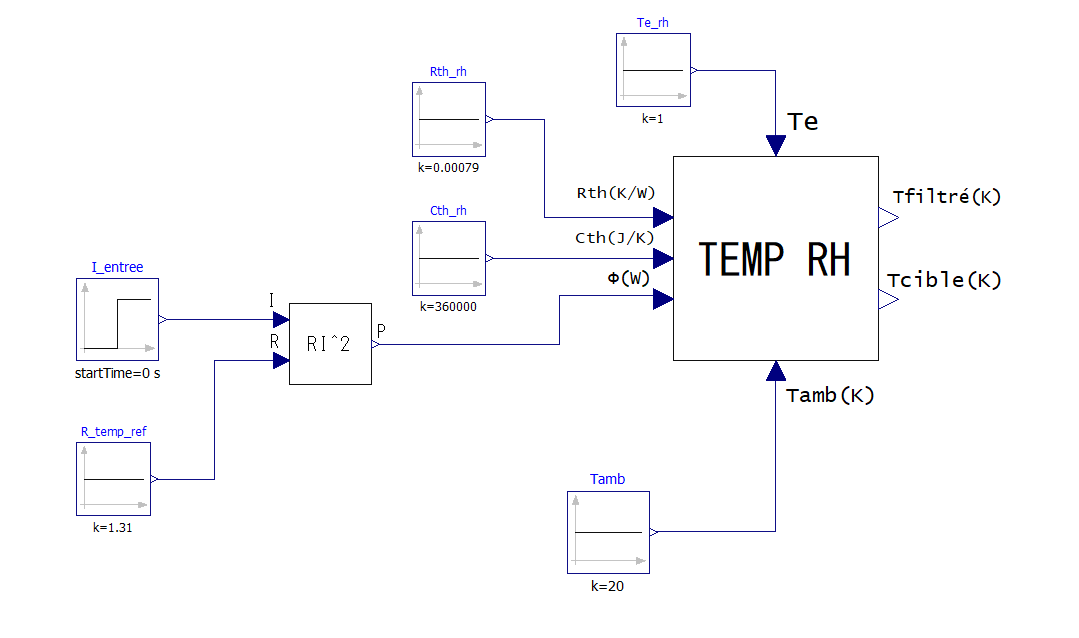
\includegraphics[width=0.9\linewidth]{rh_modelica}
			\caption{Bloc intégré dans le projet de simulation}
			\label{fig:subim2}
		\end{subfigure}
		
		\caption{création d'un bloc sous OpenModelica}
		\label{fig:image2}
	\end{figure}

		
	Sans considérer la correction de la résistance du rhéostat, on peut observer que la simulation faite sur OpenModelica de la réponse à un indice de 600kW (figure \ref{modelica:result}) est très semblable à la courbe fournie par le constructeur (figure \ref{data:result}).
	\begin{figure}[h]			
		\centering
		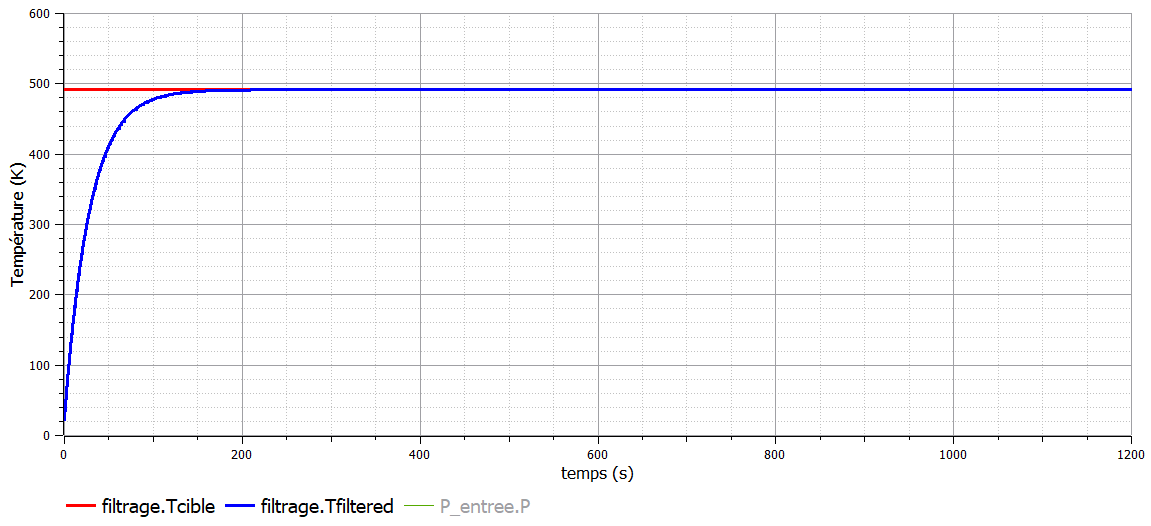
\includegraphics[width=0.6\textwidth]{rh_modelica_result}
		\caption{réponse à un échelon de courant: simulation}
		\label{modelica:result}
		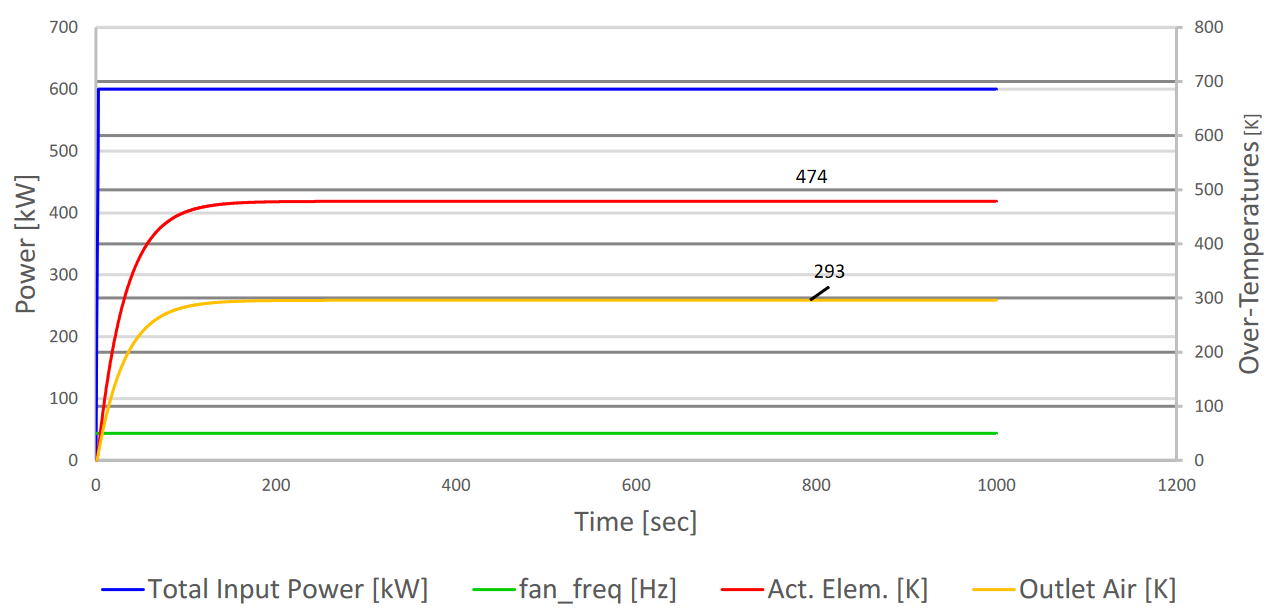
\includegraphics[width=0.6\textwidth]{rh_data_result}
		\caption{réponse à un échelon de courant: données du constructeur}
		\label{data:result}
	\end{figure}
	\pagebreak % PAGE BREAK !!! ------------------------------------------------- PAGE BREAK !!!
	On peut dans un second temps créer un nouveau bloc réalisant la correction de la résistance (cf. figure \ref{fig:subim2_1}). Dans les mêmes conditions de simulation que précédemment, on observe que la résistance corrigée atteint une valeur de 1.62 $\Omega$ (cf. figure \ref{fig:subim2_2}) et la température du rhéostat est de 290°C au lieu de 180°C lorsqu'on n'applique pas la correction.
	\begin{figure}[h]
		
		\begin{subfigure}{0.5\textwidth}
			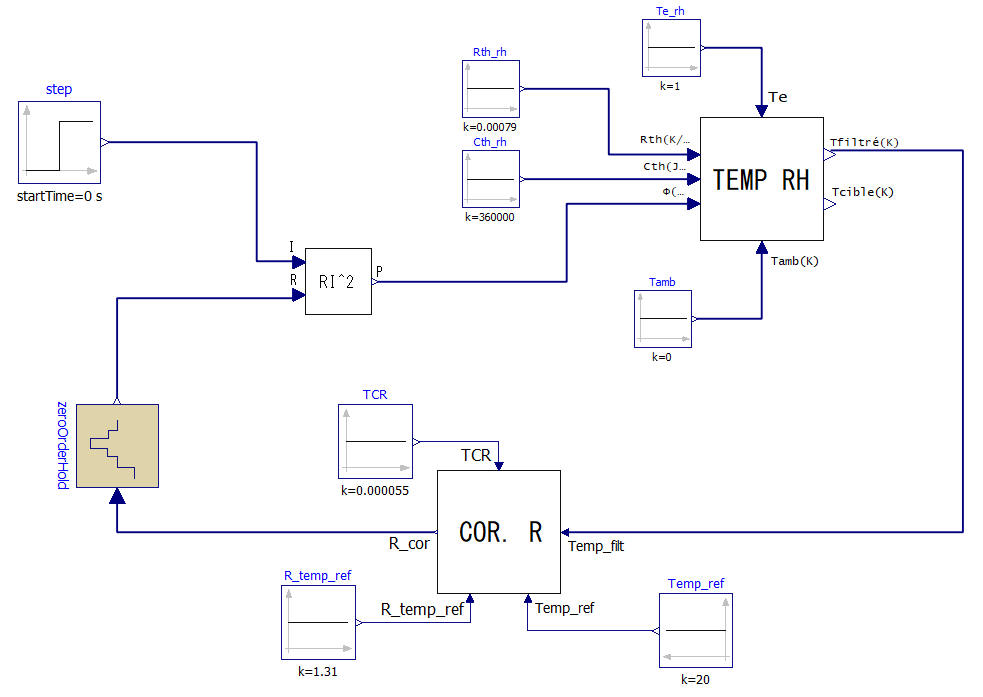
\includegraphics[width=0.9\linewidth]{rh_modelica_rcor} 
			\caption{Vue du système avec correction de résistance}
			\label{fig:subim2_1}
		\end{subfigure}
		\begin{subfigure}{0.5\textwidth}
			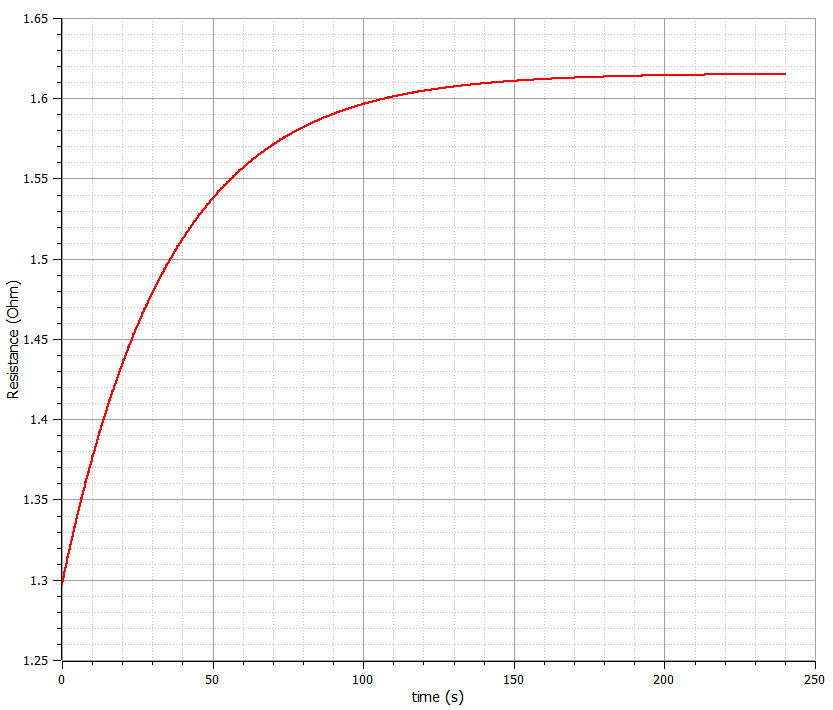
\includegraphics[height=5.5cm]{rcor_result}
			\caption{Variation de la résistance en réaction à un échelon de 600kW}
			\label{fig:subim2_2}
		\end{subfigure}
		\caption{Correction de la résistance}
		\label{fig:image2_2}
	\end{figure}
	
	Ces premiers résultats montrent la validité du modèle. On continue maintenant vers la programmation sous ControlBuild.
	
	\pagebreak % PAGE BREAK !!! ------------------------------------------------- PAGE BREAK !!!

	\subsection{Codage du modèle en ST sous ControlBuild}
	
	%	La première étape est de créer un nouveau composant au bon endroit dans l'arborescence du projet dans lequel je travaille. On s'aperçoit ainsi que toutes les fonctions du train (de l'ouverture d'une porte jusqu'à commande des freins) sont présentes et rattachées à leur TCU respectif dans les différents "coffres de traction". Dans notre cas, le modèle de rhéostat s'intègre dans le coffre "auxiliaire" \textbf{précision}.\\
	
	Pour programmer en ST, ControlBuild a quelques particularités dans son utilisation. Par exemple, les variables ne sont pas déclarées dans le code mais dans un outil séparé de la fenêtre de programmation. En plus du nom et du type, on doit aussi préciser si la variable est une entrée, une sortie ou une variable locale. Mal utiliser (ex: assignation d'une variable d'entrée) ou ne pas utiliser une variable mène à une erreur de compilation.\\
	Cette rigueur imposée par l'environnement de développement est optimisée pour des applications favorisant la sécurité comme c'est le cas dans le ferroviaire.\\
	
	En plus du fonctionnement de base du modèle, on ajoute quelques fonctionnalités pour s'accorder avec les spécifications:
	\begin{itemize}
		\item Le système sélectionne l'une des trois vitesses de ventilation.	
		
		\item L'utilisateur a le choix du nombre d'éléments du rhéostat en série.	
		
		\item Pour un effort de freinage constant, on doit avoir une puissance constante dissipée dans le rhéostat. Or, plus on dissipe de puissance, plus la température augmente dans le rhéostat et plus sa valeur en Ohm augmente. La puissance étant calculée avec cette valeur de résistance, on observe une augmentation de la puissance alors que le courant en entrée du courant est resté le même. Pour empêcher ce problème, il faut que le calculateur adapte la commande du hacheur délivrant le courant au rhéostat. On décide donc d'effectuer la correction de la résistance et l'acquisition du courant à une période supérieure à celle de l'exécution du programme de façon à donner du temps au hacheur d'effectuer une correction du courant. Cette période Te doit pouvoir être choisie par l'utilisateur au moyen d'une variable d'entrée.
		
		\item Pour le calcul de la puissance, l'utilisateur a le choix d'utiliser la valeur instantanée du courant échantillonnée à tous les Te ou d'utiliser une valeur moyennée sur Te. La sélection de ce paramètre se fait avec une variable booléenne en entrée.
		
		\item A des fin de test, on souhaite être en mesure de réaliser plusieurs forçages:
		\begin{itemize}
			\item Désactivation du composant. La température en sortie prend la valeur 0 et la valeur de résistance corrigée prend la valeur de résistance en entrée. L'utilisateur ne peut plus agir sur le modèle.
			\item Forçage de la résistance. La résistance n'est pas corrigée par le modèle et prend la valeur de résistance en entrée avec possibilité d'action de l'utilisateur.
			\item Forçage de la température cible issue de la loi de Fourier permettant d'émettre une valeur de résistance modifiée.
			\item Choix de contourner l'étape de filtrage de la température.
		\end{itemize}
		
	\end{itemize}
	
	Sans entrer dans les détails, le programme est structuré comme suit :
	
	\begin{figure}[h]			
		\centering
		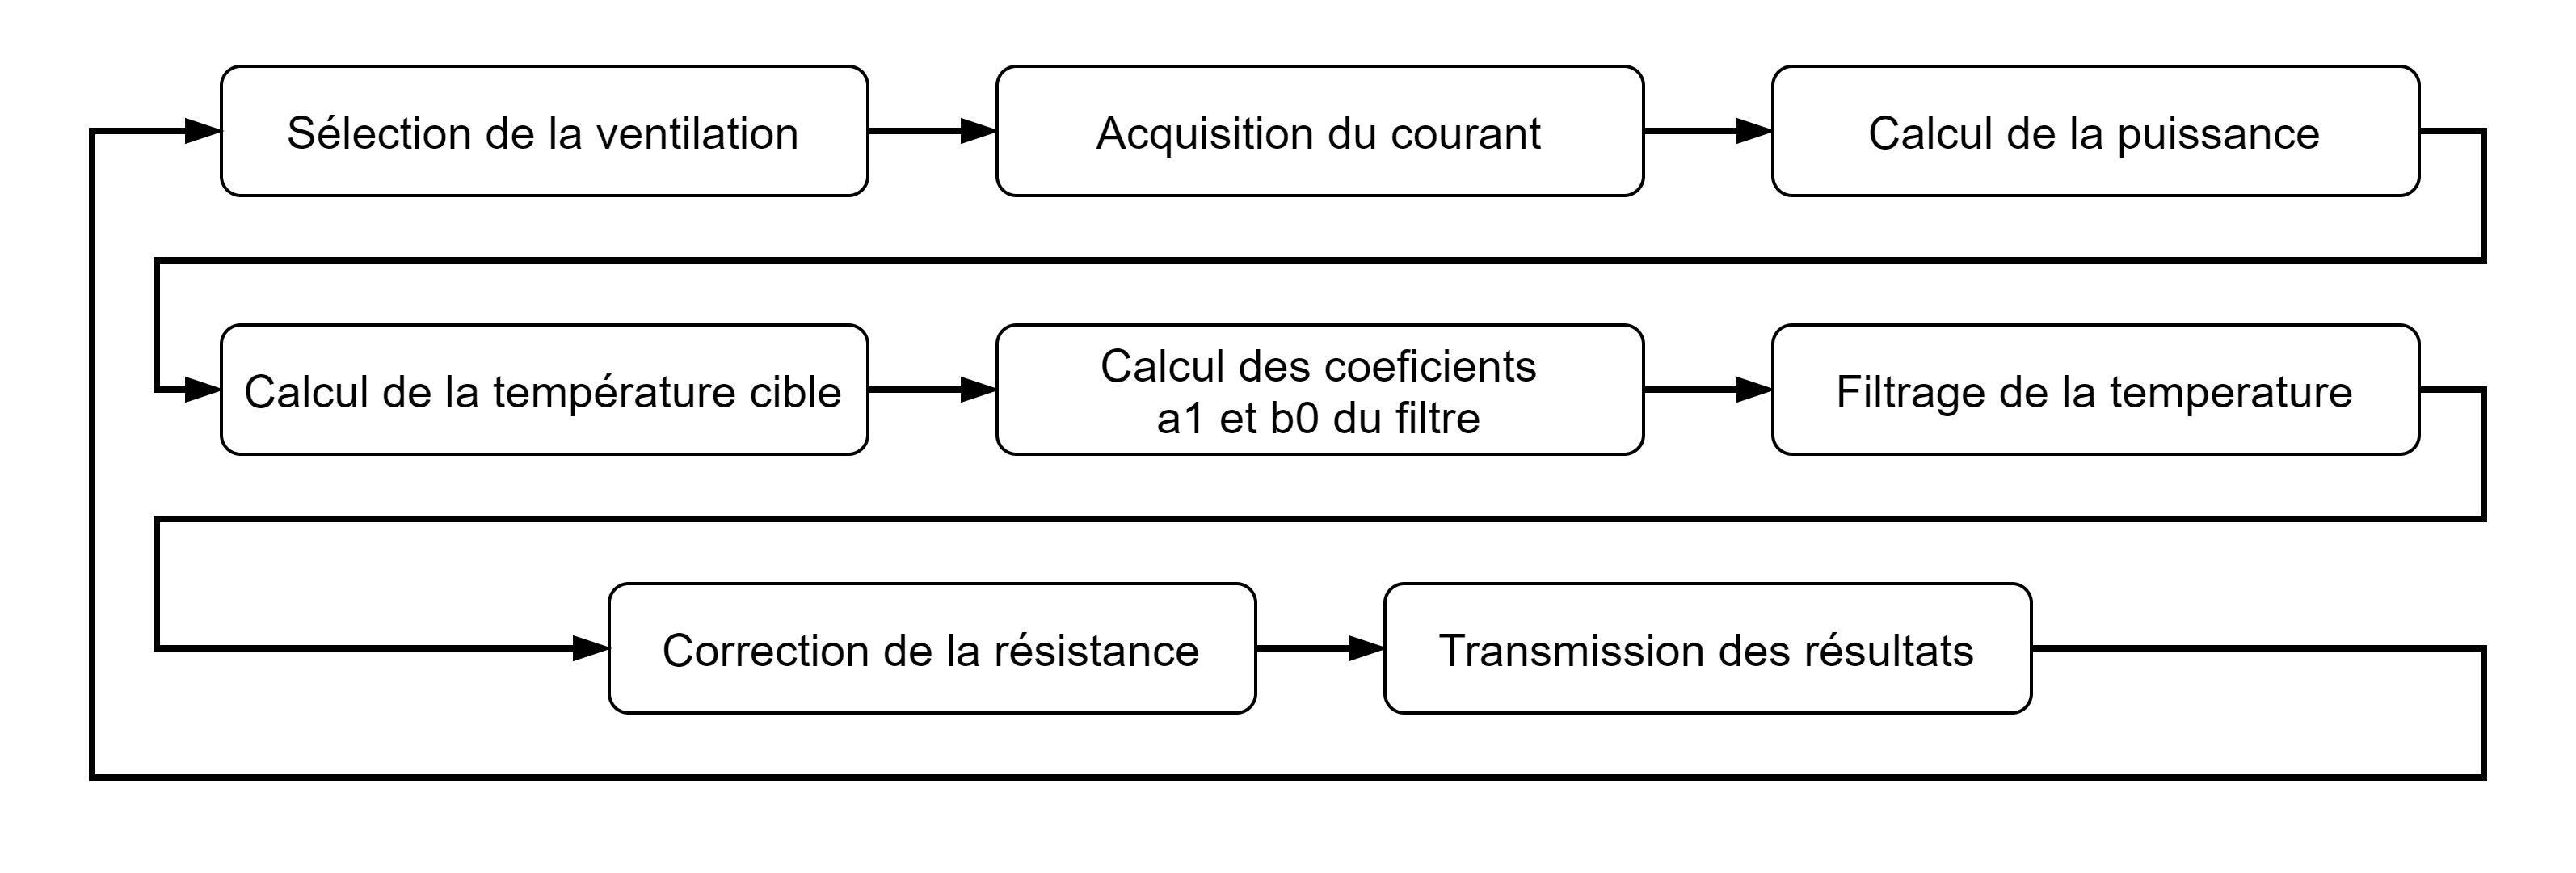
\includegraphics[width=0.8\textwidth]{schema_programme}
		\caption{structure du programme}
		\label{schema:programme}
	\end{figure}
	
	
	\pagebreak % PAGE BREAK !!! ------------------------------------------------- PAGE BREAK !!!
	
	\subsection{Tests et interprétation des résultats}
	Le test du modèle passe par la rédaction d'une procédure. Il s'agit de vérifier les différentes fonctionnalités (modes de forçages) ainsi que la validité (les résultats sont-ils cohérents ?).\\
	
	Dans un premier temps, on fait des tests en simulation PC, c'est-à-dire depuis son poste et isolé des autres composants. Les modifications des variables ne peuvent être faites que par l'utilisateur. Ensuite, le composant est intégré au projet global et testé sur simulateur. Cette fois-ci, c'est le calculateur qui communique avec la simulation, on est alors capable de voir le comportement du modèle en autonomie.\\
	
	 
	\subsection{Conclusion}
	Malgré la simplicité de ce modèle, les résultats sont cohérents avec les relevés du banc de test. Le code pourra donc être exploité par le service Contrôle-Commande afin de valider leurs programmes. 
	Nous allons pouvoir mettre à l'épreuve ce modèle dans une nouvelle application, la simulation thermique d'un transformateur de puissance.
	
	\pagebreak % PAGE BREAK !!! ------------------------------------------------- PAGE BREAK !!!
		
	\section{Modèle thermique du transformateur principal}
	\subsection{Introduction}
	On souhaite simuler la température d'un transformateur de puissance afin d'appréhender les risques de surchauffe pouvant endommager l'appareil.
	Le transformateur principal prend la tension de la caténaire et l'abaisse à ses différents secondaires (dans notre situation, un secondaire par moteur de traction) pour ensuite les redresser. Il est immergé dans un circuit d'huile forcé par une pompe et refroidi par un échangeur à air (classe KDAF : liquide forcé, air forcé) (cf. figure \ref{schema:transfo}). L'échangeur est refroidi par une ventilation fonctionnant à deux vitesses.\\
	
		\begin{figure}[h]
		\centering
		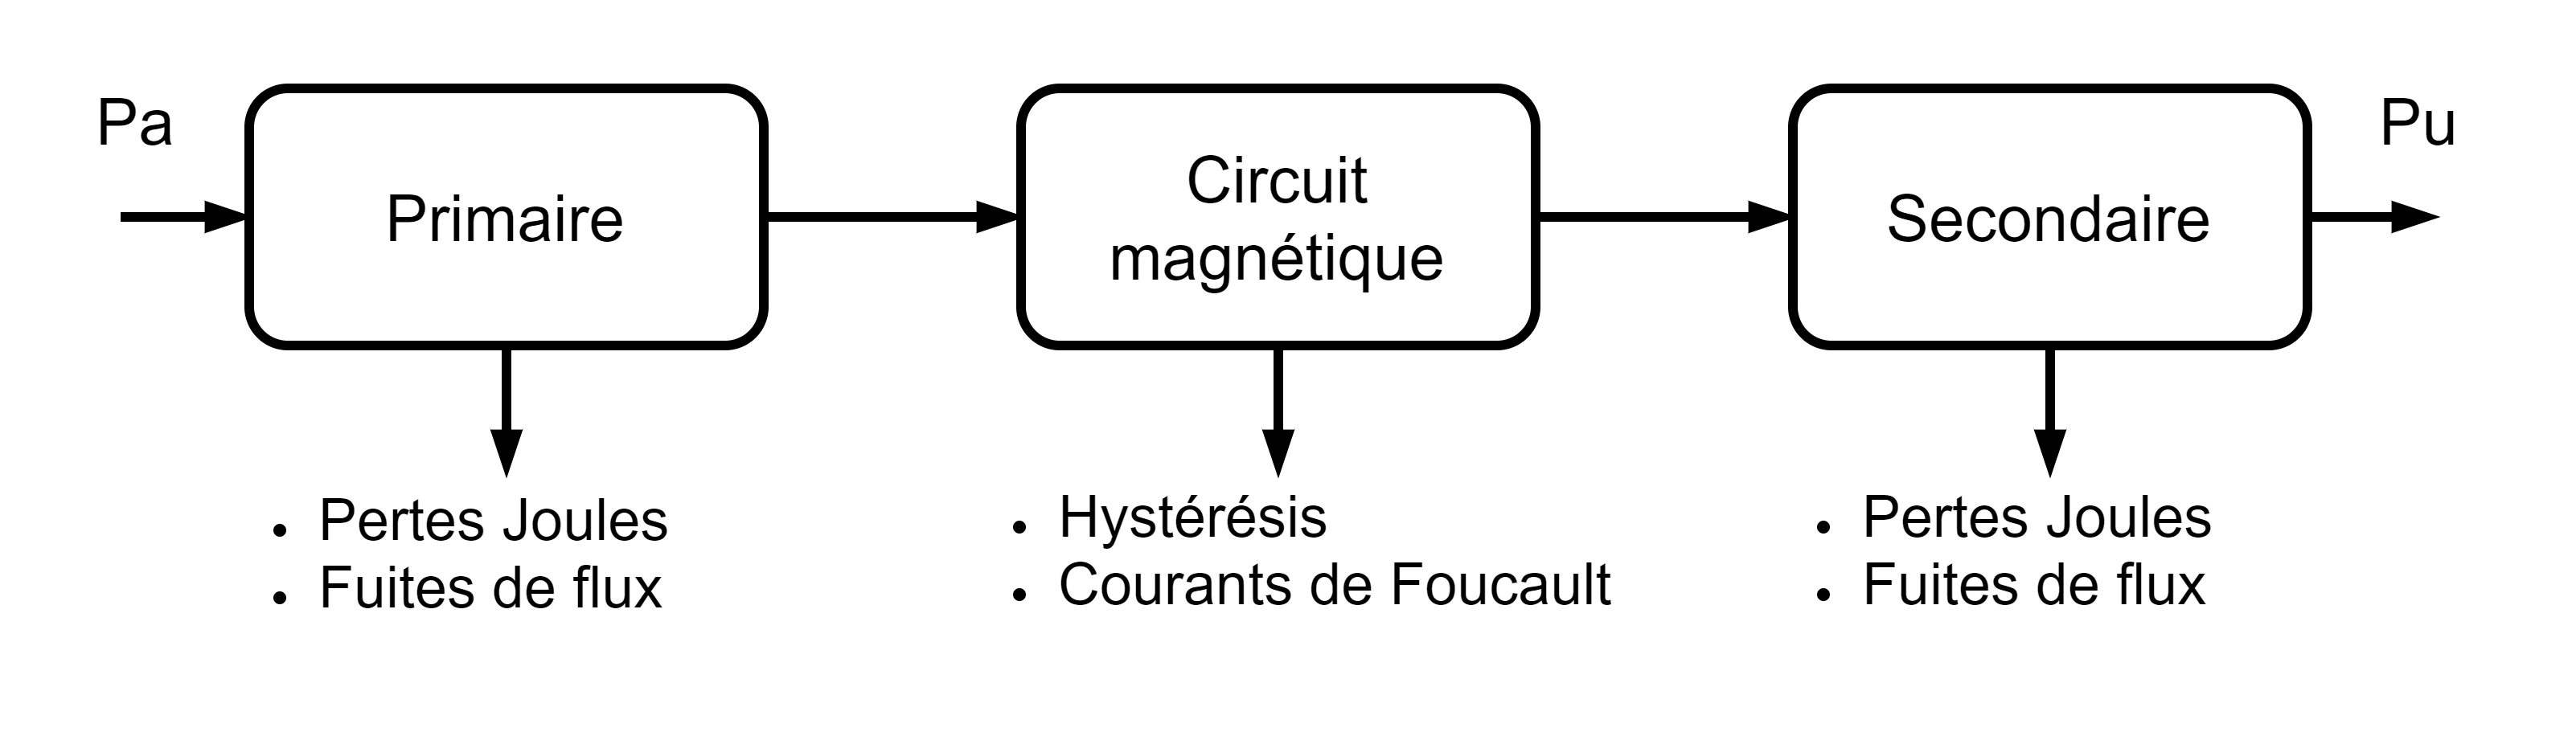
\includegraphics[width=0.6\textwidth]{schema_ptransfo}
		\caption{sources de pertes dans un transformateur}
		\label{schema:ptransfo}
	\end{figure}

	Afin de simplifier ce modèle et pour le faire correspondre à celui déjà élaboré pour le rhéostat de freinage, on fait l'hypothèse que toutes les pertes du transformateurs (cf. figure \ref{schema:ptransfo}) sont regroupées en un seul "générateur de flux". Également, cette simplification est faite pour l'échangeur.
	Ce modèle prend en entrée la puissance dissipée issue de la mesure. Est produite en sortie la température de l'huile et des enroulement du transformateur. 



	
	\begin{figure}[h]
		\centering
		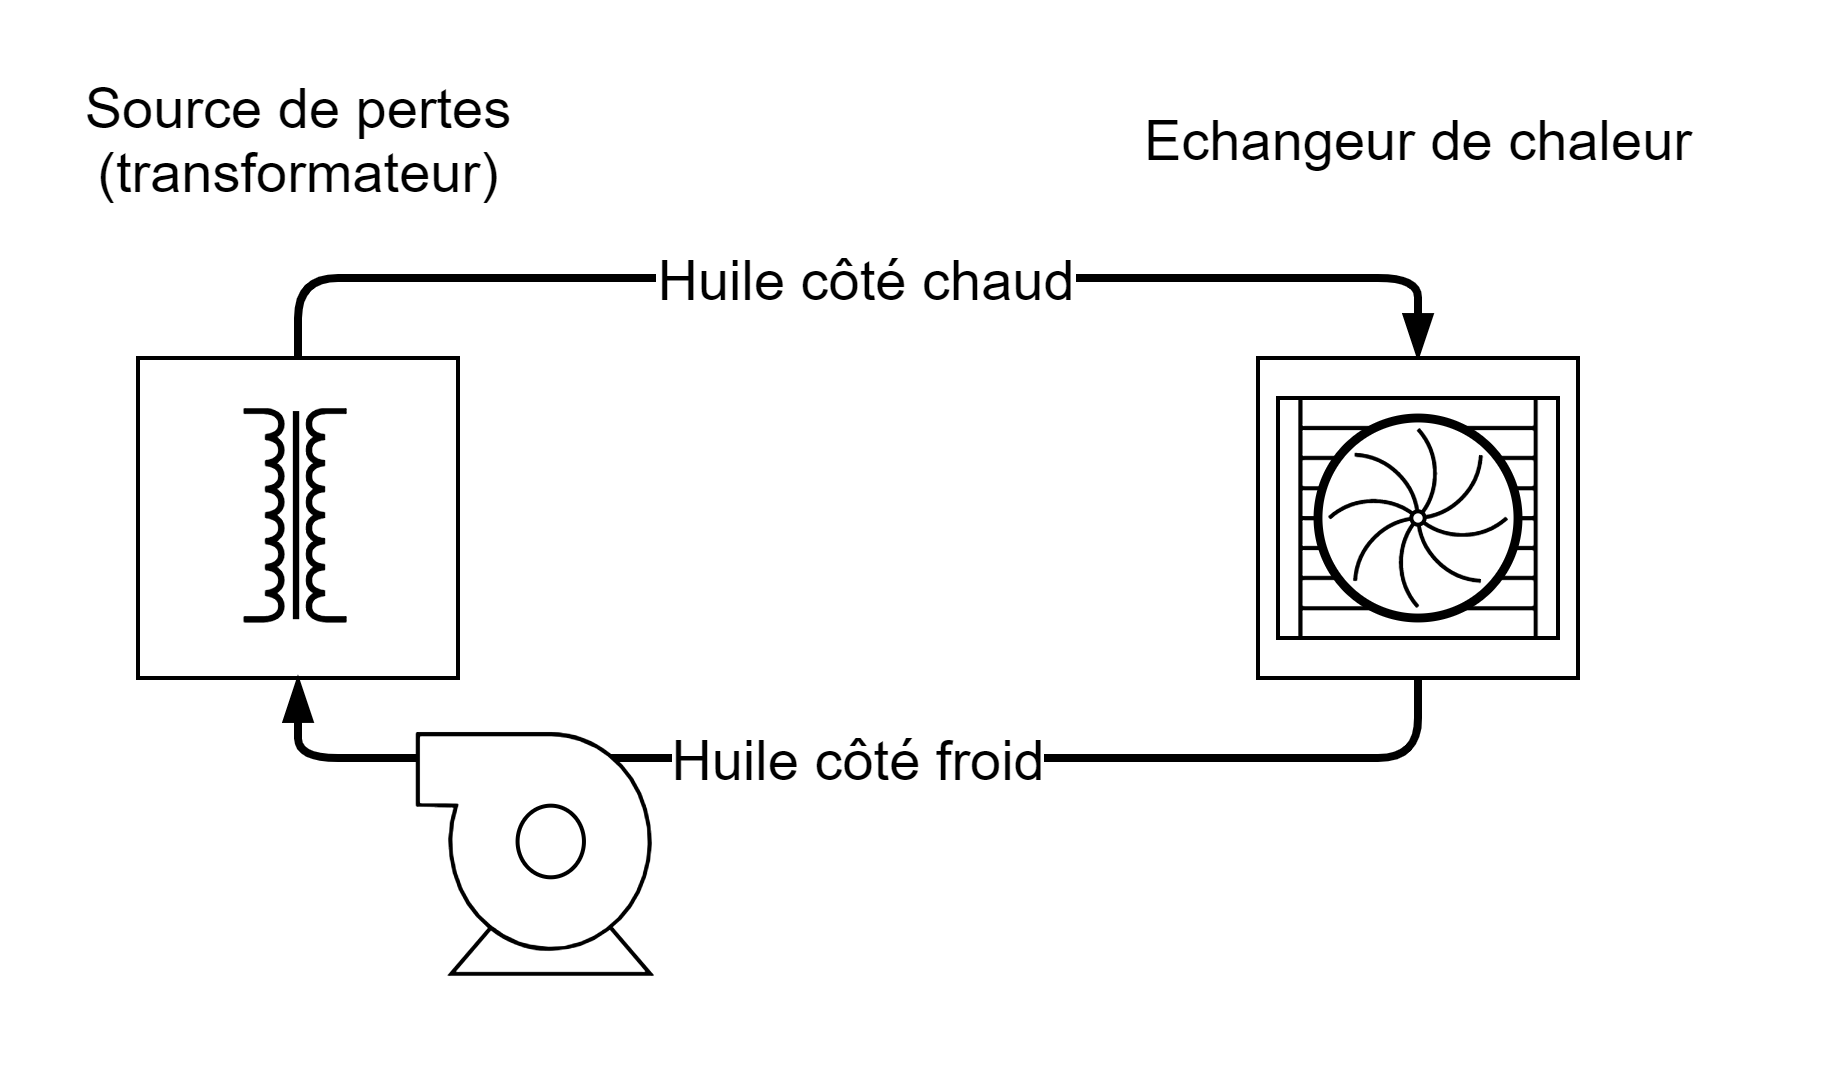
\includegraphics[width=0.5\textwidth]{schema_transfo}
		\caption{transformateur dans son circuit de refroidissement}
		\label{schema:transfo}
	\end{figure}
	
	
	Dans l'application transformateur, la majorité des échanges thermiques sont de la conduction. Le transfert entre un élément solide comme le fer ou le cuivre et l'huile peut être considéré comme de la conduction puisque ils sont conçus pour faire un bon contact et favoriser l'échange. Pour les transferts au sein de l'huile (la chaleur est transmise à l'intérieur de l'huile pour atteindre l'échangeur), le processus n'est pas entièrement linéaire. Les transferts dans l'huile font intervenir de la conduction et de la convection.\\
	La circulation de l'huile est forcée au moyen d'une pompe, on peut considérer être dans un cas de convection forcée et utiliser la loi de Newton. Il faut alors définir les coefficients de convection appropriés afin de calculer une résistance thermique équivalente.\\
	
	\subsection{Revue des données techniques}
	
	On cherche des informations relatives au comportement thermique du transformateur.
	\begin{itemize}
		\item Capacité de ventilation:
		\begin{itemize}
			\item Demi vitesse : 95kW
			\item Pleine vitesse : 190kW
		\end{itemize}
		\item Température maximale du conducteur : 130°C
		\item Pertes à vide : 3kW
		\item Type d'huile : Ester 
	\end{itemize}
	On s'aperçoit qu'à la différence des données du rhéostat, on ne dispose pas de résistances thermiques et capacités thermiques. Malgré cela, on se propose de poursuivre avec l'élaboration du modèle pour ensuite le mettre à l'épreuve avec les valeurs manquantes.\\
	
	\subsection{Modelisation sous OpenModelica}
	
	L'idée 
	
	La simulation du Transformateur principal réutilise le composant créé pour le modèle de rhéostat ainsi qu'une version légèrement modifiée ne réalisant que le filtrage. Le modèle est composé de cinq fonctions:
	\begin{itemize}
		\item Le bloc "cuivre" génère une température en fonction des pertes dissipées.
		\item Le bloc "huile chaude" représente un point médian entre le cuivre et l'échangeur. Il ne change pas l'amplitude du flux de chaleur à régime établi mais ne fait que le filtrer.
		\item La commande de la ventilation observe température de l'huile chaude et active ou désactive la ventilation selon un cycle d'hystérésis.
		\item "échangeur" est modélisé par le même bloc que "cuivre" à la différence que le flux entrant dans le bloc est négatif, ce qui génère une température négative et permet le refroidissement.
		\item "huile froide", comme "huile chaude" représente un point milieu entre la face froide de l'échangeur et le cuivre.
	\end{itemize}
	\begin{figure}[h]
		\centering
		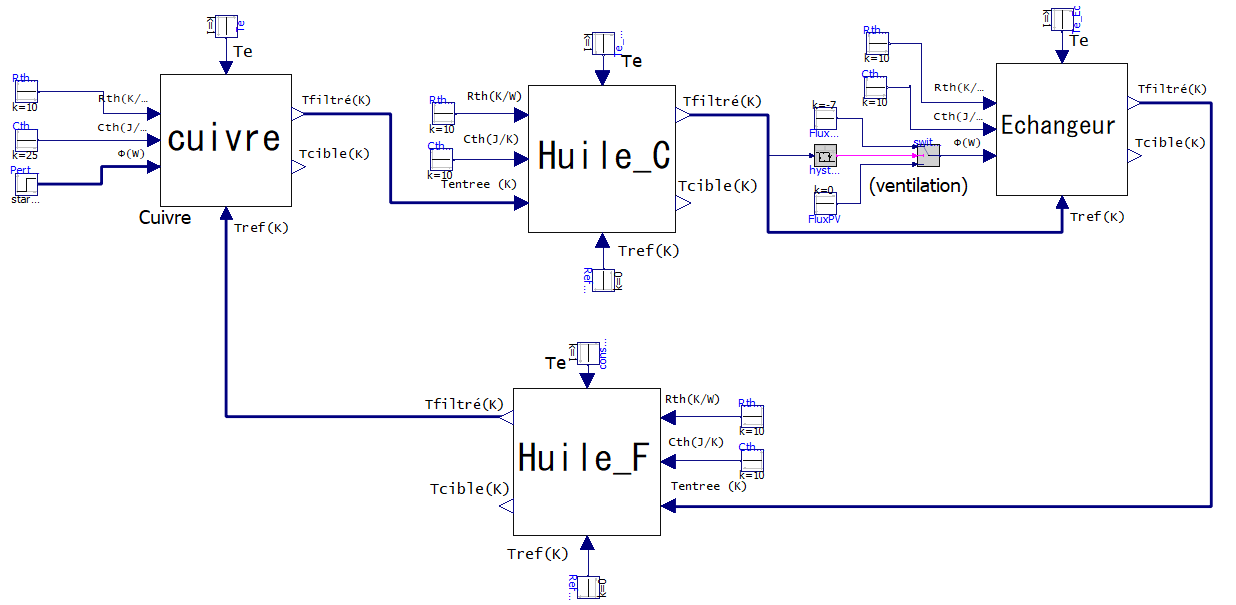
\includegraphics[width=0.75\textwidth]{tfp_modelica}
		\caption{Système transformateur complet}
		\label{tfp:modelica}
	\end{figure}
	% --------------------------------------------------- FIN DÉVELOPPEMENT	
	\chapter{Valorisation du stage par rapport au projet d'insertion}
	% --------------------------------------------------- DÉBUT CONCLUSION
	
		Ce stage m'a permis de réaliser un modèle thermique simple mis en œuvre pour la simulation des chaînes de traction ferroviaires.
		Cela m'a permis de développer mes compétences techniques. Associant des connaissances en électrotechnique et en programmation, j'ai pu mettre en œuvre des connaissances acquises en DUT GEII ainsi qu'en Licence Professionnelle CCRSEE.\\
	
		En effet, j'ai pu me rendre compte au long de ce stage que les deux formations que j'ai suivies à l'IUT de Tarbes sont très liées aux domaines dans lesquels évolue Alstom. \\
		
		Pendant ce stage, si j'ai souvent eu l'occasion de communiquer avec l'équipe, j'ai majoritairement travaillé en autonomie. Cela a été l'occasion de m'écarter de l'organisation du travail en équipe dont j'ai fait l'expérience à de multiples reprises au cours des projets d'études et réalisation de DUT et du projet tuteuré en Licence Professionnelle.\\
	
		Dans le cadre de mon projet professionnel, j'ai pu acquérir une expérience dans la programmation des systèmes embarqués et en particulier d'un simulateur de chaîne de traction ce qui m'encourage à poursuivre dans ce milieu.\\
		
		Je me suis senti très bien accueilli à Alstom et en particulier dans mon service où j'ai pu faire l'expérience d'une ambiance de travail à la fois très professionnelle et très humaine.\\
		
		J'ai trouvé très enrichissant de communiquer avec les personnes de mon service au sujet du parcours professionnel et universitaire de chacun. Je me suis rendu compte de l'importance d'être à l'aise dans son environnement de travail et d'apprécier la compagnie des collègues en dehors du contexte strictement professionnel.
		Ce stage m'a conforté dans l'idée de travailler dans une grande structure comme Alstom.\\
		
		Pour finir, je tiens à dire que je conserve une très bonne impression de cette courte expérience dans le domaine du ferroviaire.\\

	 
	
	% --------------------------------------------------- FIN CONCLUSION
	\renewcommand{\bibname}{Références} % changement du titre des chapitres en "parties"
	\begin{thebibliography}{9}
		
		
		\bibitem{transfer_thermique_pspice} 
		Shuhui Li, Rajab Challoo et Robert A. McLauchlan. 
		\textit{Heat Transfer Simulation Using PSpice}.\\ 
		Conference: ASME 2003 Heat Transfer Summer Conference.\\
		DOI:10.1115/HT2003-47021
		
		\bibitem{brake_resistor} 
		Thomas B. D. Björklund. 
		\textit{A brake resistor perspective on Thermal Management}.\\ 
		CDanotherm Electric [En ligne]. 2015 [consulté le 26 mars 2021].\\
		Disponible sur: \\\texttt{https://www.danotherm.com/power-resistors/downloads}
		
		\bibitem{histoire_alstom} 
		\textit{Génèse et Histoire du site Alstom à Séméac}.\\
		Maire de Soues. [En ligne]. 2014 [consulté le 20 mai 2021].\\
		Disponible sur: \\\texttt{https://www.soues.com/Fichiers/pages/155333145124genese-et-histoire-du-site-alstom-a-semeac.pdf}
		
		\bibitem{ACTGV_pmcf} 
		\textit{PMCF Onduleurs}.\\
		Association des Conducteurs de Trains à Grande Vitesse. [En ligne] M.Durochat et G.Desplanques [consulté le 05 juin 2021].\\
		Disponible sur: \\\texttt{http://actgv.fr/wp-content/uploads/2012/05/PMCF-onduleur.pdf}
		
		\bibitem{ACTGV_puissance} 
		\textit{Circuits de Puissance Traction}.\\
		Association des Conducteurs de Trains à Grande Vitesse. [En ligne] M Durochat, Jean Willemin et G. Desplanques, 2016 [consulté le 03 juin 2021].\\
		Disponible sur: \\\texttt{http://actgv.fr/wp-content/uploads/2016/10/Circuit-de-Puissance-21-04-2016-dernier-travail.pdf}
		
		\bibitem{alstom_site} 
		\textit{Site officiel d'Alstom}.\\
		Site officiel d'Alstom. [En ligne] [consulté le 08 juin 2021].\\
		Disponible sur: \\\texttt{https://www.alstom.com}
		
	\end{thebibliography}
	
	
\end{document}